%%% The main file. It contains definitions of basic parameters and includes all other parts.

% Meta-data of your thesis (please edit)
\input metadata.tex

% Generate metadata in XMP format for use by the pdfx package
\input xmp.tex

%% Settings for single-side (simplex) printing
% Margins: left 40mm, right 25mm, top and bottom 25mm
% (but beware, LaTeX adds 1in implicitly)
\documentclass[12pt,a4paper]{report}
\setlength\textwidth{145mm}
\setlength\textheight{247mm}
\setlength\oddsidemargin{15mm}
\setlength\evensidemargin{15mm}
\setlength\topmargin{0mm}
\setlength\headsep{0mm}
\setlength\headheight{0mm}
% \openright makes the following text appear on a right-hand page
\let\openright=\clearpage

%% Settings for two-sided (duplex) printing
% \documentclass[12pt,a4paper,twoside,openright]{report}
% \setlength\textwidth{145mm}
% \setlength\textheight{247mm}
% \setlength\oddsidemargin{14.2mm}
% \setlength\evensidemargin{0mm}
% \setlength\topmargin{0mm}
% \setlength\headsep{0mm}
% \setlength\headheight{0mm}
% \let\openright=\cleardoublepage

%% If the thesis has no printed version, symmetric margins look better
% \documentclass[12pt,a4paper]{report}
% \setlength\textwidth{145mm}
% \setlength\textheight{247mm}
% \setlength\oddsidemargin{10mm}
% \setlength\evensidemargin{10mm}
% \setlength\topmargin{0mm}
% \setlength\headsep{0mm}
% \setlength\headheight{0mm}
% \let\openright=\clearpage

%% Generate PDF/A-2u
\usepackage[a-2u]{pdfx}

%% Prefer Latin Modern fonts
\usepackage{lmodern}
% If we are not using LuaTeX, we need to set up character encoding:
\usepackage{iftex}
\ifpdftex
\usepackage[utf8]{inputenc}
\usepackage[T1]{fontenc}
\usepackage{textcomp}
\fi

%% Further useful packages (included in most LaTeX distributions)
\usepackage{amsmath}        % extensions for typesetting of math
\usepackage{amsfonts}       % math fonts
\usepackage{amsthm}         % theorems, definitions, etc.
\usepackage{bm}             % boldface symbols (\bm)
\usepackage{booktabs}       % improved horizontal lines in tables
\usepackage{caption}        % custom captions of floating objects
\usepackage{dcolumn}        % improved alignment of table columns
\usepackage{floatrow}       % custom float environments
\usepackage{graphicx}       % embedding of pictures
\usepackage{indentfirst}    % indent the first paragraph of a chapter
\usepackage[nopatch=item]{microtype}   % micro-typographic refinement
\usepackage{paralist}       % improved enumerate and itemize
\usepackage[nottoc]{tocbibind} % makes sure that bibliography and the lists
			    % of figures/tables are included in the table
			    % of contents
\usepackage{xcolor}         % typesetting in color

% The hyperref package for clickable links in PDF and also for storing
% metadata to PDF (including the table of contents).
% Most settings are pre-set by the pdfx package.
\hypersetup{unicode}
\hypersetup{breaklinks=true}

% Packages for computer science theses
\usepackage{algpseudocode}  % part of algorithmicx package
\usepackage{algorithm}
\usepackage{fancyvrb}       % improved verbatim environment
\usepackage{listings}       % pretty-printer of source code

% You might want to use cleveref for references
% \usepackage{cleveref}

% Set up formatting of bibliography (references to literature)
% Details can be adjusted in macros.tex.
%
% BEWARE: Different fields of research and different university departments
% have their own customs regarding bibliography. Consult the bibliography
% format with your supervisor.
%
% The basic format according to the ISO 690 standard with numbered references
\usepackage[natbib,style=iso-numeric,sorting=none]{biblatex}
% ISO 690 with alphanumeric references (abbreviations of authors' names)
%\usepackage[natbib,style=iso-alphabetic]{biblatex}
% ISO 690 with references Author (year)
%\usepackage[natbib,style=iso-authoryear]{biblatex}
%
% Some fields of research prefer a simple format with numbered references
% (sorting=none tells that bibliography should be listed in citation order)
%\usepackage[natbib,style=numeric,sorting=none]{biblatex}
% Numbered references, but [1,2,3,4,5] is compressed to [1-5]
%\usepackage[natbib,style=numeric-comp,sorting=none]{biblatex}
% A simple format with alphanumeric references:
%\usepackage[natbib,style=alphabetic]{biblatex}

% Load the file with bibliography entries
\addbibresource{bibliography.bib}

% Our definitions of macros (see description inside)
\input macros.tex

%%% Title page and various mandatory informational pages
\begin{document}
%%% Titulní strana práce a další povinné informační strany

%%% Nápisy na přední straně desek
%%% Pokud je práce ve slovenštině, desky mají být česky.

% Desky obvykle nesázíme, ale pokud je chcete přidat, změnte \iffalse na \iftrue
\iffalse

\pagestyle{empty}
\hypersetup{pageanchor=false}
\begin{center}

\large
Univerzita Karlova

\medskip

Matematicko-fyzikální fakulta

\vfill

{\huge\bf\ThesisTypeTitle}

\vfill

{\huge\bf\ThesisTitle\par}

\vfill
\vfill

\hbox to \hsize{\YearSubmitted\hfil \ThesisAuthor}

\end{center}

\newpage\openright
\setcounter{page}{1}

\fi

%%% Titulní strana práce
%%% Pokud je práce ve slovenštině, tato strana zůstává česky.

\pagestyle{empty}
\hypersetup{pageanchor=false}

\begin{center}

\centerline{\mbox{\includegraphics[width=166mm]{img/logo-cs.pdf}}}

\vspace{-8mm}
\vfill

{\bf\Large\ThesisTypeTitle}

\vfill

{\LARGE\ThesisAuthor}

\vspace{15mm}

{\LARGE\bfseries\ThesisTitle\par}

\vfill

\Department

\vfill

{
\centerline{\vbox{\halign{\hbox to 0.45\hsize{\hfil #}&\hskip 0.5em\parbox[t]{0.45\hsize}{\raggedright #}\cr
Vedoucí \ThesisTypeGenitive{} práce:&\Supervisor \cr
\ifx\ThesisType\TypeRig\else
\noalign{\vspace{2mm}}
Studijní program:&\StudyProgramme \cr
\fi
}}}}

\vfill

Praha \YearSubmitted

\end{center}

\newpage

%%% Strana s čestným prohlášením k práci
%%% Pokud je práce ve slovenštině, tato strana zůstává česky.

\openright
\hypersetup{pageanchor=true}
\vglue 0pt plus 1fill

\noindent
Prohlašuji, že jsem tuto \ThesisTypeAccusative{} práci vypracoval(a) samostatně a výhradně
s~použitím citovaných pramenů, literatury a dalších odborných zdrojů.
Beru na~vědomí, že se na moji práci vztahují práva a povinnosti vyplývající
ze zákona č. 121/2000 Sb., autorského zákona v~platném znění, zejména skutečnost,
že Univerzita Karlova má právo na~uzavření licenční smlouvy o~užití této
práce jako školního díla podle §60 odst. 1 autorského zákona.

\vspace{10mm}

\hbox{\hbox to 0.5\hsize{%
V \hbox to 6em{\dotfill} dne \hbox to 6em{\dotfill}
\hss}\hbox to 0.5\hsize{\dotfill\quad}}
\smallskip
\hbox{\hbox to 0.5\hsize{}\hbox to 0.5\hsize{\hfil Podpis autora\hfil}}

\vspace{20mm}
\newpage

%%% Poděkování

\openright

\noindent
\Dedication

\newpage

%%% Povinná informační strana práce

\openright
{\InfoPageFont

\vtop to 0.5\vsize{
\setlength\parindent{0mm}
\setlength\parskip{5mm}

Název práce:
\ThesisTitle

Autor:
\ThesisAuthor

\DeptType:
\Department

Vedoucí \ThesisTypeGenitive{} práce:
\Supervisor, \SupervisorsDepartment

Abstrakt:
\Abstract

Klíčová slova:
{\def\sep{\unskip, }\ThesisKeywords}

\vfil
}

\vtop to 0.49\vsize{
\setlength\parindent{0mm}
\setlength\parskip{5mm}

Title:
\ThesisTitleEN

Author:
\ThesisAuthor

\DeptTypeEN:
\DepartmentEN

Supervisor:
\Supervisor, \SupervisorsDepartmentEN

Abstract:
\AbstractEN

Keywords:
{\def\sep{\unskip, }\ThesisKeywordsEN}

\vfil
}

}

\newpage

%%% Další stránky budeme číslovat
\pagestyle{plain}


%%% A page with automatically generated table of contents of the thesis

\tableofcontents

%%% Each chapter is kept in a separate file
\chapter*{Used terms}
\addcontentsline{toc}{chapter}{Used Terms}
\chapter*{Introduction}
\addcontentsline{toc}{chapter}{Introduction}

\section*{Motivation}

Every social network with userbase past a certain threshold will at some point face a problem.
The problem is in essence a question of filtering.
Questions like what should we show to our users, in what order or how often have to be answered at the very least by every big-tech company.

And the amount of data to consider can be vast.
Meta-owned social apps for example, have over 3.29 billion daily active users as of september 2024 \cite{metaDau2024}.
\xxx{TODO - naučit se citovat}
When different tastes and preferences of the userbase are to be taken into account
this problem becomes a very interesting software engineering challenge indeed.

It's safe to say that all the big contemporary social networks (Facebook, Twitter (newly rebranded to X), Instagram, Reddit or TikTok)
tackle this challenge in the same way.
Commonly reffered to as "The algorithm",
their solutions rely on machine learning to learn user preferences and maximize retention time.

And the result? User gets presented with an infinite feed of content
with another tweet, picture or video just a scroll away.

This approach while for sure effective at maximizing ad revenue and user retention has its downsides:
\begin{itemize}
  \item Users have little conscious control over the content they see. The algorithm decides for them based on nebulous criteria.
  \item Echo chambers - the algorithm will show the user more of what they like and agree with making it easy to believe that
  everyone thinks the same way.
  \item The process of using the app can easily become addictive as each swipe is akin to pulling a lever on a slot machine.
\end{itemize}
While subjective, I believe that these are common experiences of users of social networks.

\section*{Afantázie}
Afantázie is the implementation part and the final product of this thesis.
It's a website (currently hosted on domain afantazie.cz)
on which I'm going to attempt to give an alternative to how we interact with social networks.

This alternative is a graph-based approach where
users are presented with a graph of nodes representing posts and edges representing connections between them.

Now ideally user could log in and see the entirety of the content on the website.
This is of course unfeasable not only from technical perspective but also because of limits of human perception.
Our eyes and brains can only process so much information at once
and rendering potentially billions of nodes is even bigger challenge than the aforementioned infinite feed approach.

But I believe there is a way to make this idea work.
While seeing the entirety of the content is practically impossible,
giving users the ability to see currently relevant content as a graph might be feasable.
If we also add the ability to zoom and dynamically load more content related to the area of interest (ie. zoomed-in coordinates of the graph),
this approach might become a viable way to interact with at least smaller-scale social networks.

If implemented properly, this solution could solve the problems mentioned:
\begin{itemize}
  \item Users would have more control over the content they see. They could zoom in on the parts of the graph they find interesting.
  \item Echo chambers could be mitigated by showing the user the graph-based context of the entire site.
  \item While from the perspective of software makers, an addictive product is not a bad thing, it's not necessarily good for the users.
    Graph-based interaction doesn't rely on addictive patterns and if in anyway adictive,
    the addictiveness would stem from exploring the content on users own terms.
\end{itemize}

\xxx{To wrap up this introduction, I'm going to present a picture TODO. It's the header of a news article called 72 Hours of Gamergate}

The task ahead is going to require solving technical challenges regarding development and hosting of a public website
as well as implementation and research about graph vizualization.

I will start by presenting and comparing a few existing software products that provide graph visualization,
then I will move to graph layout algorithms that make these visualizations possible and finally I will implement the website itself.
\chapter{Graph Layout Algorithms}
\label{chap:graph_layout_algorithms}

Graph layout algorithms (or \glspl{GLA} for short) are a class of algorithms used for computing positions
of nodes so that they make a nice-looking or helpful diagram.
These algorithms accept graph-representing data as input and produce positions of individual nodes as output.

In this work, we are going to assume that GLAs produce 2-dimensional layouts,
but it is worth mentioning that the number of dimensions can be arbitrarily high.

There are many types of GLA, each with its strengths and weaknesses.
Let us look at some of the common ones.

\section{Circular Layout}

Circular layout (Figure \ref{obr:graph_layout_circular}) algorithms arrange nodes in a circle, often emphasizing the structure of the graph by placing nodes
with similar properties close together.
In a circular layout, nodes can be distributed evenly along the circumference of the circle,
or their placement can be weighted by specific properties (e.g., node degree or importance).

\begin{figure}[p]\centering
    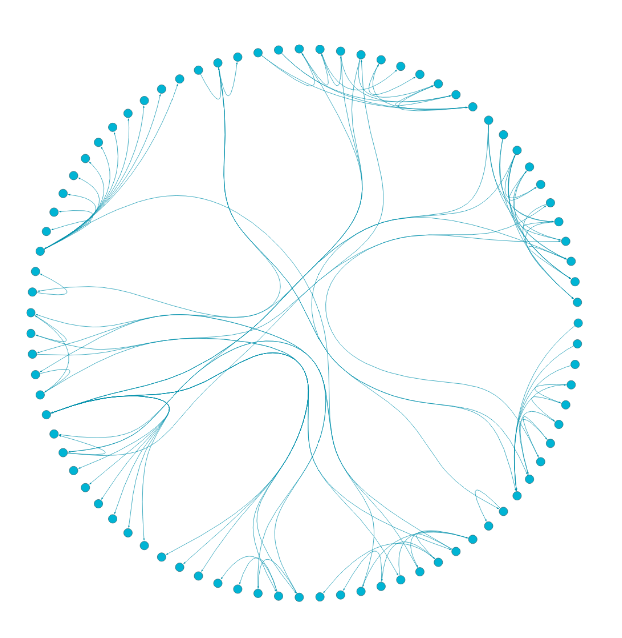
\includegraphics[width=140mm, keepaspectratio]{img/graph_layout_cicrular.png}
    \caption{Circular layout\cite{graph_layout_demos}}
    \label{obr:graph_layout_circular}
\end{figure}

\section{Hierarchical Layout}

Hierarchical layout (Figure \ref{obr:graph_layout_hierarchical})algorithms are designed to emphasize directional relationships, such as those found in flowcharts,
dependency graphs, or organizational charts. These algorithms arrange nodes in layers or levels, with edges generally
flowing in a single direction (e.g., top to bottom or left to right).

This layout can be applied to general graphs but is most effective for directed acyclic graphs (DAGs) or undirected trees.
Note that the structure in Figure \ref{obr:graph_layout_radial} is not a tree but a general graph.

\begin{figure}[p]\centering
    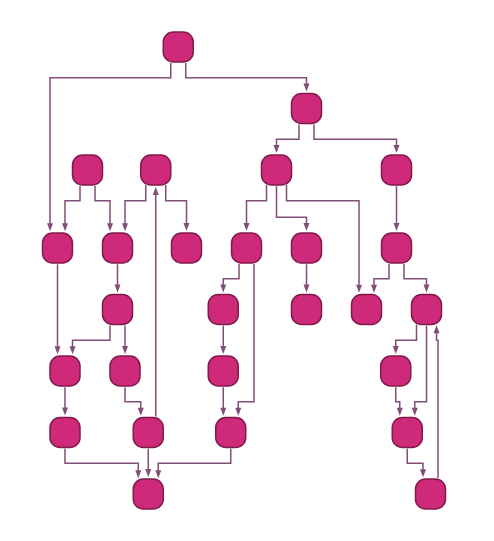
\includegraphics[width=140mm, keepaspectratio]{img/graph_layout_hiearchichal.png}
    \caption{Hierarchical layout\cite{graph_layout_demos}}
    \label{obr:graph_layout_hierarchical}
\end{figure}

\section{Radial Layout}

Radial layout (Figure \ref{obr:graph_layout_radial}) is a type of hierarchical layout where nodes are arranged in concentric circles around a central node (root).
Its immediate neighbors are arranged in the first circle. Subsequent layers represent nodes further away.
Radial layout can help highlight relationships between the central node and its surroundings.

Figure \ref{obr:graph_layout_radial} shows a tree.
In the context of social networks, many of the contemporary social networks are composed of trees:
\begin{itemize}
    \item \textbf{Reddit} - The root represents a post, and the rest are its comments
    \item \textbf{Twitter} - The root is a standalone tweet, and the rest form a series of replies
    \item \textbf{Youtube} - The root is a video, and the rest are its comments
\end{itemize}

As such, if one visualized the content of these social networks, it might look like a set of radial layouts.
We are highlighting this fact because Aphantasia's content structure is not a \gls{tree} but a \gls{DAG}
which might have interesting consequences for navigation, user experience, and usage.

\begin{figure}[p]\centering
    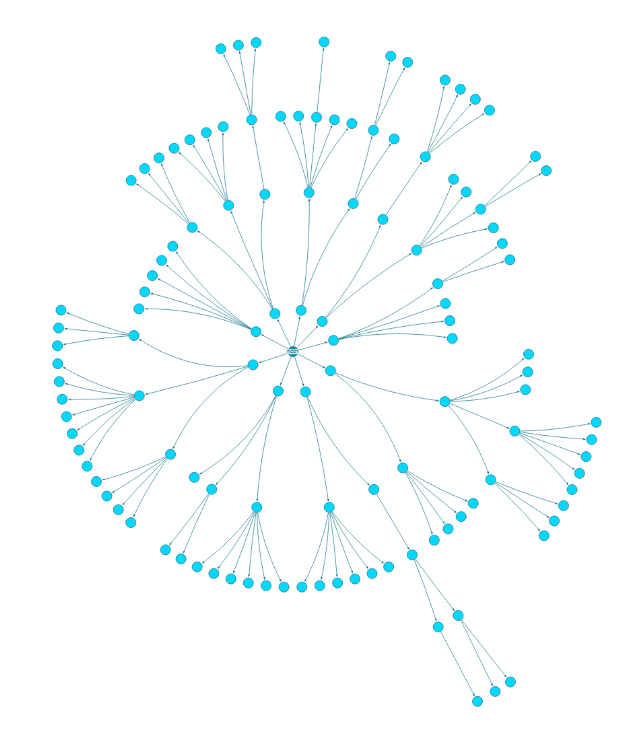
\includegraphics[width=140mm, keepaspectratio]{img/graph_layout_radial.png}
    \caption{Radial layout\cite{graph_layout_demos}}
    \label{obr:graph_layout_radial}
\end{figure}

\section{Force-Directed Layout}
\label{sec:force_directed_layout}

This type of layout is going to be the focus of this work.
All of the layouts we will see in Chapter \ref{chap:related_software} were produced by force-directed layout (FDL) algorithms.

The main idea behind FDL algorithms is very intuitive:
Nodes are attracted to each other when connected by an edge and repelled otherwise.
Elegant in concept and easy to implement, this approach is endlessly customizable.

One particularly useful feature is that FDL algorithms are incremental and update the layout continuously.
This can be utilized to produce visually pleasing animations of the data and allows for user interaction
(e.g., dragging nodes around or changing parameters).
The dragging feature can also be used to aid the algorithm in achieving a more desired layout during its run.

Thanks to this aspect, a developer implementing an FDL algorithm has the ability to adjust the strength of the forces, add new ones,
or implement entirely new behaviors and parameters to fit specific use cases 
- all by watching the animation run, interacting with it, and inferring what behavior needs to be changed or added.

These positives are, however, balanced by two drawbacks:
\begin{itemize}
    \item high time complexity

 The basic version of FDL has a time complexity of $O(n^2)$ per step, where $n$ is the number of nodes in the graph.
 For stabilization, usually $n$ steps are considered sufficient,
 and thus, the time complexity for producing a stabilized graph is often computed as $O(n^3)$.

    \item sensitive parameterization
    
 As for parameterization, the algorithm is highly dependent on the parameters set by the user (or developer),
 some of which can be very sensitive and radically change the resulting layout with only a small change in value.
 This can be a challenge for users unfamiliar with the algorithm or the data they are working with.
 Achieving a specific look or quality for the final graph render often requires a significant amount of time spent tweaking the parameters.

 This fact also means that it is difficult to create a "one size fits all" FDL algorithm
 - the parameters that work well for one dataset might not work well for another.
\end{itemize}
\chapter{Graph Layout Algorithms}

Graph layout algorithms (or GLAs for short) are a class of algorithms used for computing positions
of nodes so that they make a nice or useful diagram.
These algorithms accept graph-representing data as input and produce positions of individual nodes as output.

In this work, we are going to assume that GLAs produce 2-dimensional layouts,
but it is worth mentioning that the number of dimensions can be arbitrarily high.

There are many types of GLAs, each with its own strengths and weaknesses. Let'S look at some of the common ones.

\section{Circular Layout}

Circular layout (figure \ref{obr:graph_layout_circular}) algorithms arrange nodes in a circle, often emphasizing the structure of the graph by placing nodes
with similar properties close together.
In a circular layout, nodes can be distributed evenly along the circumference of the circle,
or their placement can be weighted by certain properties (e.g., node degree or importance).

\begin{figure}[p]\centering
    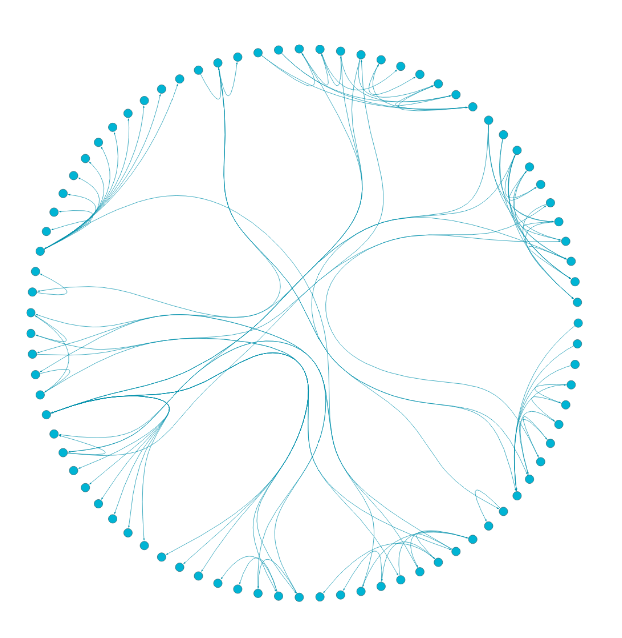
\includegraphics[width=140mm, keepaspectratio]{img/graph_layout_cicrular.png}
    \caption{Circular layout\cite{graph_layout_demos}}
    \label{obr:graph_layout_circular}
\end{figure}

\section{Hierarchical Layout}

Hierarchical layout (figure \ref{obr:graph_layout_hierarchical})algorithms are designed to emphasize directional relationships, such as those found in flowcharts,
dependency graphs, or organizational charts. These algorithms arrange nodes in layers or levels, with edges generally
flowing in a single direction (e.g., top to bottom or left to right).
This layout can be applied to general graphs but is most effective for directed acyclic graphs (DAGs) or undirected trees.

\begin{figure}[p]\centering
    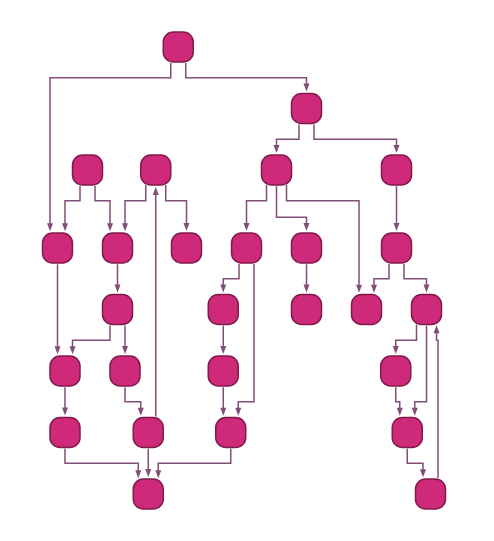
\includegraphics[width=140mm, keepaspectratio]{img/graph_layout_hiearchichal.png}
    \caption{Hierarchical layout\cite{graph_layout_demos}}
    \label{obr:graph_layout_hierarchical}
\end{figure}

\section{Radial Layout}

Radial layout (figure \ref{obr:graph_layout_radial}) is a type of hierarchical layout where nodes are arranged in concentric circles around a central node.
Its immediate neighbors are arranged in the first circle. Subsequent layers represent nodes further away.
Radial layout can help highlight relationships between the central node and its surroundings.

\begin{figure}[p]\centering
    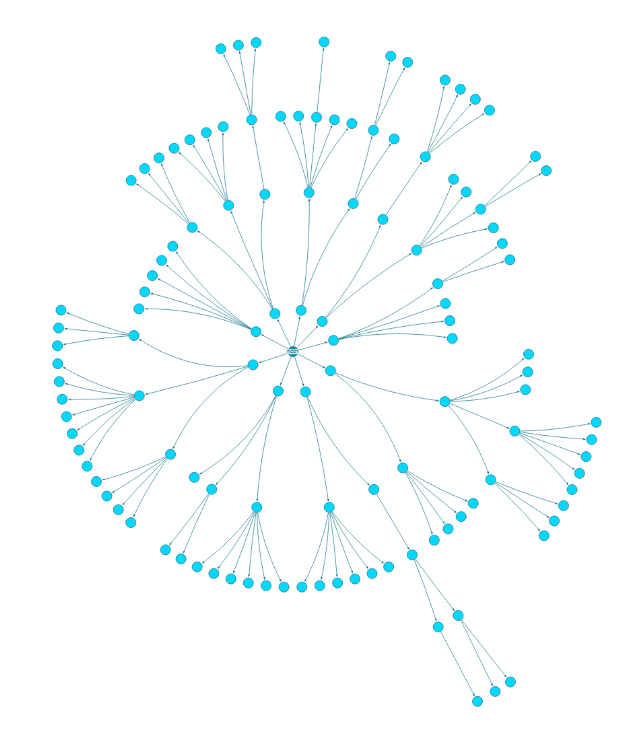
\includegraphics[width=140mm, keepaspectratio]{img/graph_layout_radial.png}
    \caption{Radial layout\cite{graph_layout_demos}}
    \label{obr:graph_layout_radial}
\end{figure}

\section{Force-Directed Layout}
All graph layouts we saw in chapter 1 were produced by force-directed layout (FDL) algorithms.
\footnote{We weren't able to find any specifics about the algorithm used in Obsidian.
However, from the way its graph view behaves, it is safe to assume a variation of an FDL algorithm was used.}

The main idea behind FDL algorithms is very intuitive:
nodes are attracted to each other when connected by an edge and repelled otherwise.
Elegant in concept and easy to implement, this approach is endlessly customizable.

One particularly useful feature is that FDL algorithms are incremental and update the layout continuously.
This can be utilized to produce visually pleasing animations of the data and allows for user interaction
(e.g., dragging nodes around or changing parameters).
The draging feature can also be used to aid the layout algorithm towards a more desired layout.

Thanks to this aspect, a developer implementing an FDL algorithm has the ability to adjust the strength of the forces, add new ones,
or implement entirely new behaviors and parameters to fit specific use cases 
- all by watching the animation run, interacting with it and inferring what behavior needs to be changed or added.

These positives are, however, balanced by two drawbacks:
\begin{itemize}
    \item high time complexity

    The basic version of FDL has a time complexity of $O(n^2)$ per step, where $n$ is the number of nodes in the graph.
    For stabilization, usually $n$ steps are considered sufficient,
    and thus the time complexity for producing a stabilized graph is often computed as $O(n^3)$.

    \item sensitive parameterization
    
    As for parameterization, the algorithm is highly dependent on the parameters set by the user (or developer),
    some of which can be very sensitive and radically change the resulting layout with only a small change in value.
    This can be a challenge for users who are not familiar with the algorithm or the data they are working with.
    Achieving a specific look or quality for the final graph render often requires time spent tweaking the parameters.
\end{itemize}
\chapter{Software design}

\section{Requirements and use-cases}

\section{Technologies and architecture}

\section{Utilized algorithms}

\section{Data structures}

\section{Plan of execution}
\chapter{Implementation}
\label{chap:implementation}
In this chapter, we will go through the implementation process of Aphantasia and the technical challenges we faced.
The relevant source code is available at \url{https://github.com/0rbit3r/afantazie_bachelors_thesis}.

\section{Preparation}

Aphantasia will be a publicly accessible web application, and as such, we will need to set up the following:
\begin{itemize}
  \item \textbf{Frontend} - a webpage serving an interactive graph and UI
  \item \textbf{Backend} - for business logic and data processing
  \item \textbf{Database} - for persistence of data
  \item \textbf{Hosting} - to make the website accessible
\end{itemize}

\subsection{Used Technologies and Libraries}
Before implementing Aphantasia, we need to decide on the technologies we will utilize.

\subsubsection{Hosting, Database and Backend}
Let us start from the bottom with hosting.
We will use a Virtual Private Server (VPS) from a hosting company, Váš Hosting.
They will provide us with a Linux server fully prepared for hosting, including
SSL certificates, domains, databases, and tools to manage the server.

For the backend, we will use \textbf{.NET 8.0} with \textbf{C\#}.
While the main reason for this decision is familiarity with the technology, the .NET platform is regardles as a good choice as:
\begin{itemize}
    \item It is Linux-compatible
    \item The provided the \textbf{Entity Framework Core} library provides \gls{ORM}, complete \gls{code_first} solutions and makes it easy to replace database technology later on if needed
\end{itemize}

For the database, we will use \textbf{PostgreSQL} (version 15.10) as it is one of the most popular database engines and is known for its reliability and performance.
We will use \gls{code_first} approach to database design and will use Entity Framework Core (version 8.0.4) to scaffold and migrate the database
(programmatically create and update the database schema based on defined Entities in the project).

\subsubsection{Graph View}
This is where the most crucial decisions will be made as its graph view is the our primary focus and we are striving for a good user experience.

We already saw a library that might be usable in our case in Section \ref{sec:cytoscape_js}.
We decided against using it as we would use only a fraction of its features, and it might be overkill for our needs.
Instead, we will implement our own graph rendering engine using a custom \gls{GLA}
implementation and render the nodes using a rendering library.

The reasoning behind this is primarily based on customizability
- we will be able to implement only the features we need and optimize the rendering for our use case.

To render the graph, we will use an existing JavaScript library capable of 2D graphics.
We considered four possibilities to render the graph:
\begin{itemize}
    \item \textbf{HTML and CSS} - the most barebones solution would be to use a set of divs to represent nodes and SVG lines to represent edges
    \item \textbf{HTML5 Canvas} - a more sophisticated solution to draw both nodes and edges in HTML5 Canvas API
    \item \textbf{PixiJS} - library for 2D rendering in the browser
    \item \textbf{Three.js} - library for 3D rendering in the browser
\end{itemize}

We chose to use \textbf{PixiJS} (version 7.4.2) as it seemed to provide a good compromise between ease of use and performance for 2D rendering in the browser.

\subsubsection{Pages and UI}
To implement graph view UI and pages for user management, login, and post creation, it makes sense to take advantage of a JavaScript framework.
We have experience with two - Angular and React.

We will use \textbf{React} (version 18.2.0) with TypeScript.
React has an unopinionated approach to architecture, which should make it easier to integrate with our rendering solution.
We have already seen that React can be integrated with Cytoscape.js in Section \ref{sec:cytoscape_js}.
We will attempt to integrate React with PixiJS to create a graph view page with UI controls friendly on both desktop and mobile devices.

\subsection{Plan of Execution}
With technological decisions made, the roadmap for the implementation of Aphantasia is as follows:

\begin{enumerate}
    \item In the first stage (Section \ref{sec:basic_web_app}), we will implement a basic web application, including user management.
 We will host this application on the VPS, set up a PostgreSQL database, and configure the reverse proxy server.

    \item Next, in Section \ref{sec:small_graph_implementation} we will implement small graph rendering engine. 
 The result of this stage should contain an Obsidian-like graph view capable of rendering at least a few hundred nodes.

    \item And lastly, in Section \ref{sec:big_graph_implementation}, we will extend the application to handle large graphs and thus finish the implementation.
\end{enumerate}

\section{Basic Web Application}
\label{sec:basic_web_app}
In this section we will describe our process of creating a simple web application, scaffold the backend architecture, set up the database and implement user management.
We also decided to implement a simple chat service during this phase.
The reasoning behind this decision was the following:
\begin{itemize}
    \item It will serve as preparation for the real-time server-client communication, which will be useful for the graph view
 (see Section \ref{sec:server_client_communication})
    \item The user management system, just on its own, is not useful or testable
    \item The chat is locked behind login, and thus, we can develop and test authorization early on
    \item The messages inherit the color of their author, and thus, we can test the color selection feature
\end{itemize}

\subsection{Database Schema}
We set up the database of Aphantasia, including the graph-specific tables:
\begin{itemize}
    \item \textbf{Users} - holds the user data
    \item \textbf{Thoughts} - holds the thought data
    \item \textbf{ThoughtReferences} - holds the links between the thoughts
\end{itemize}

A diagram of the database schema can be seen in Figure \ref{obr:afantazie_database_schema}.
\begin{figure}[h]\centering
    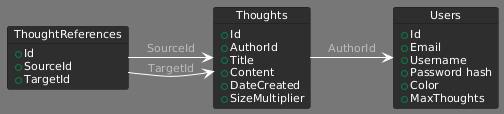
\includegraphics[width=140mm]{img/afantazie_database_schema.png}
    \caption{Aphantasia Database schema}
    \label{obr:afantazie_database_schema}
\end{figure}

We created the database using \gls{code_first} approach and scaffolded the local development database and production database using Entity Framework Core.
With that, the database is ready to be used by the backend.

\subsection{Backend Architecture}
\label{sec:implementation_backend}
The backend of the basic application is an ASP.NET application written in C\#.
Similarly to the database schema, we decided to develop architectural design early on and it paid off as development of later features was much easier. 
The initial architectural blueprint remained mostly unchanged until the end of the project.

The solution of the backend consists of 19 projects implementing the backend to Aphantasia and one project for secondary tools
(see Section \ref{sec:testing_data} for more details). 

The backend projects are divided into four directories (forming conceptual layers):
\begin{itemize}
    \item \textbf{Presentation}
    \item \textbf{Service}
    \item \textbf{Core} 
    \item \textbf{Data}
\end{itemize}

There is also one project outside of these layers that serves to Bootstrap the application and set up \gls{dependency_injection}.
Figure \ref{obr:afantazie_backend_architecture} describes the architecture of the backend with its dependencies.

This division is loosely based on Onion architecture \cite{onion_architecture}. Notice that the Presentation layer doesn't directly depend on the Service layer.
Instead, it depends on the Service Interface layer, and the actual implementation is injected at runtime.
This allows for clean separation of concerns, makes the code more testable, and allows for easy swapping of implementations.

\begin{figure}[h]\centering
    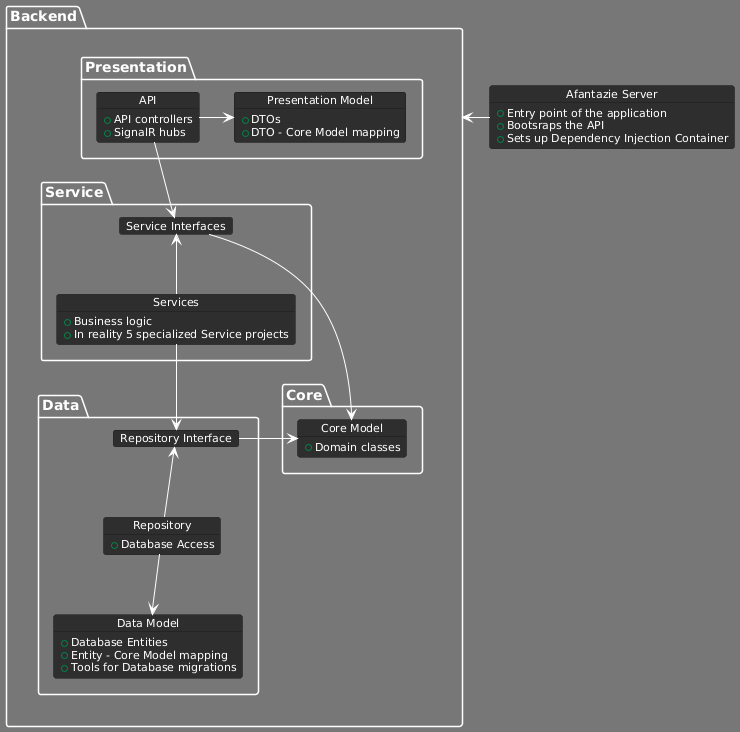
\includegraphics[width=140mm]{img/backend_architecture.png}
    \caption{Aphantasia Backend Architecture}
    \label{obr:afantazie_backend_architecture}
\end{figure}

The following sections describe the individual layers and their responsibilities in more detail.

\subsubsection*{Presentation Layer}
The Presentation layer sits in the outermost layer of the application and is responsible for handling HTTP requests and responses.
It contains two projects - \textbf{Api} and \textbf{Model}.

The Api project holds API controllers implemented using ASP.NET Core MVC.
The controllers and signalR hubs only handle incoming traffic and  
for handling \gls{business_logic}, they call the appropriate service in the Service layer.

The Presentation Model contains definitions for the data transfer objects (DTOs).
These objects are used to transfer data between the client and the server.

\subsubsection*{Service Layer}
The Service contains the \gls{business_logic} of Aphantaisa.
It is a set of 5 projects (and their respective interfaces):
\begin{itemize}
    \item \textbf{Auth} - handles user registration, login, and JWT token generation
    \item \textbf{Chat} - handles the chat functionality
    \item \textbf{Site Activity} - handles the real-time stats of the site (such as the number of users online)
    \item \textbf{Thoughts} - handles the creation and retrieval of thoughts
    \item \textbf{User Settings} - handles the user settings (such as selected color or on-screen thoughts limit)
\end{itemize}

\subsubsection*{Core Layer}
The Core contains three projects:
\begin{itemize}
    \item \textbf{Core Model} - contains the core model of the application used in Repository and Service interfaces as arguments
    \item \textbf{Localization} - contains the localization resources for the application
    \item \textbf{Constants} - contains constants (currently only the default on-screen thoughts limit for newly registered users)
\end{itemize}

This layer sits in the midle of the application dependency wise and is used by both the Service and Data layers.

\subsubsection*{Data Layer}
The Data layer is called by services to access the database using Entity Framework Core.
It contains the Repository project and its interface.
The Repository project is responsible for handling the database queries and updates.

\subsubsection*{AfantazieServer Project}
Since the application is using \gls{dependency_injection}
we cannot put its entry point inside any of the projects mentioned above without breaking the principles of the Onion architecture.
If we, for example, wanted to run the API by setting setting the Presentation.Api as the startup project, we would have to add
references to the Service layer and Data layer to add their classes to \gls{dependency_injection} container and thus break the separation of concerns.

Instead, we created a separate project that serves as the entry point for the application.
It is responsible for all the setup and configuration of the application, which includes but is not limited to:
\begin{itemize}
    \item Configuration files 
    \item Dependency injection setup
    \item CORS setup (Cross-Origin Resource Sharing)
    \item Logging setup
\end{itemize}

Note that not all of these setups are done in the AfantazieServer project itself.
All individual projects contain the bootstrapping logic, and expose an "AddModule" method that is called from the AfantazieServer project to add the respective service.
For example, the AfantazieServer project calls the AddDataModule() method from the Data project,
which then registers the Data module with all its responsibilities, allowing it to swap modules for different implementations if needed
(as long as they implement the corresponding interface).

\subsubsection*{Models}
We use three different models to represent data in the application - each serving a different purpose in its respective layer:
\begin{itemize}
    \item \textbf{Presentation Model} - DTOs used for transmission between client and server
 (The client has to implement the exact same model to be able to communicate with the server)
    \item \textbf{Data Model} - Entities correspond to Database tables
 (which is created \gls{code_first} from the entities by Entity Framework)
    \item \textbf{Core Model} - Serves as an intermediary between the Presentation and Data models.
 Business logic should be implemented in the Service layer using this model.
\end{itemize}

Both Repository and Service interfaces use the Core Model as arguments and return values.
This means that the Service layer is not dependent on either the Entities or the DTOs,
but it also requires mapping between the Core Model and the Data Model.
For mapping, we used the Mapster library inside the Data and Presentation Model projects.

\subsection{Initial Frontend Implementation}
During the first phase, we initialized the web application and implemented \gls{auth_x_y},
real-time server-client communication and routing with a few pages:
\begin{itemize}
    \item Home page
    \item Login page
    \item Registration page
    \item Chat page
    \item About page
\end{itemize}

We also styled the application using plain css. The styling is minimalistic and not exactly modern but is functional and responsive.

\subsubsection{Cache Busting}
\label{sec:cache_busting}
Browsers routinely cache files to speed up the loading of websites.
This is a good thing as it reduces the load on the server and speeds up the user experience.
However when the website is in active development and the files are changing frequently the cache can become a problem.
Users might not see the changes made to the website because the browser is loading the old cached version of the file.
The techniques for solving this problem are called Cache busting. We used a React library called React cache buster to resolve this issue.

At first, we had no success with the library as it was not working as expected.
The reason, as we found out, was that the library uses a meta.json file to store the version of the application.
The client then checks the version of the application, and if it is different from the version in the meta.json file,
it forcefully reloads the page to get the new version of the application.

The problem was that Nginx was caching the meta.json file, and the client was not getting the new version of the file.
Instead, it was getting a response with a 304 status code (not modified).
We solved this by adding a directive to the Nginx configuration file that forces the server to provide a new version of the file at all times.
See Section \ref{sec:nginx_config} for the exact configuration used.

\subsubsection{Server-Client Communication}
\label{sec:server_client_communication}
For the chat application, we tried to use \gls{websockets} for real-time communication.
While we did manage to get this approach working, we did not like the developer experience.

\textbf{SignalR} is a library that simplifies the process of setting up WebSockets and provides a nice API for server-client communication.
It is available for both .NET and JavaScript and is easy to set up, with much less boilerplate code than using WebSockets directly.

SignalR uses so-called hubs to communicate between server and client, which automatically handle
the connection and disconnection of clients.

We implemented two hubs - ChatHub and StatsHub, with the former being used for chat messages while on the chat page
and the latter used across the entire application to keep track of and display the number of users online on the homepage.

This feature can be exploited further, for example, to inform the client that new thoughts were created.

\subsection{Hosting and Server Management}
\label{sec:hosting}

The VPS we rented comes ready with a lot of tools to manage the server, is fully prepared for hosting,
is accessible via SSH and has a web-based control panel for managing the server.

After installing the .NET 8 runtime, the process of running a .NET application was as simple as transferring the program via SFTP
and inputting 'dotnet Afantazie.dll' into the terminal.
Deploying the frontend required only copying the files to the necessary directory in the server filesystem.
DNS and SSL certificates were set with a mouse click in the provided server management.

\subsubsection{Nginx}
The greatest challenge when hosting the application came with setting up a reverse proxy server (although that was mostly due to our inexperience with the technology).
Two provided reverse proxy server technologies were the default Apache and Nginx.
After a short research through forums we decided to make the switch to Nginx as it is more modern alternative to Apache and can have performance benefits.
If needed, we could always switch back to Apache without much hassle.

The provided template for the Nginx configuration was a good starting point, but in order to make the
application functional, we had to make a few additions to the afantazie.cz.conf file:
\begin{itemize}
    \item Reroute the API requests to the backend
    \item Set up redirection from HTTP to HTTPS
    \item Force the server to always provide a new version of the meta.json file used for cache busting (see Section \ref{sec:cache_busting})
\end{itemize}
For a complete configuration file, see Section \ref{sec:nginx_config}.

\section{Small Graph Vizualization}

\label{sec:small_graph_implementation}
Small graph implementation, the second phase of development, required two things - rendering and forces simulation.
As mentioned previously, we decided to render the graph using PixiJS and implement our proprietary \gls{FDL}.

To integrate PixiJS into the React application, we first followed the official documentation \cite{pixijs_official_react_guide}.
We were not happy with the result as the Pixi/react components were hard to work with programmatically.

So, instead, we used a guide by Adam Emery \cite{pixijs_adam_emery_guide} to integrate PixiJS into the React application.
His approach is different in that it only uses the Stage component from the Pixi/react library
, and the rest of the PixiJS code is written in plain JavaScript (in our case, TypeScript).
This allows us to better control the PixiJS code and use the full potential of the library instead of using the pixi/react wrapper.

After implementing a simple node and edges rendering, we quickly hit a roadblock with massive \glspl{memory_leak}.
As we found out, we were instantiating new PixiJS objects every time the graph was updated.
To mitigate this issue, we created an interface - RenderedThought - that holds the PixiJS objects for each thought (the Title text and the Circle graphics).

The RenderedThought interface remained to the end of the development and we incrementaly added more properties to it as we needed them.
It contains all the properties that are needed to render the thought on the screen and to interact with it.
For example, each rendered thought has a boolean property 'held' which is used to determine if the thought is currently being dragged by the user.

Before big graph solution we stored the loaded thoughts in an array of rendered thoughts kept in the React state.

Once we were able to render nodes and edges, we created a simple force directed layout algorithm with two forces - pull connected and push unconnected.
At this point, we had an application with a comparable graph view to obsidian (Figure \ref{obr:afantazie_selfie}).

Figure \ref{obr:afantazie_cithep_3k} showcases the first 3000 nodes of the citHep dataset now visualized using Aphantasia in this stage of development.
With this many nodes on the screen, the application lagged a lot, although it remained somewhat usable.

\begin{figure}[p]\centering
    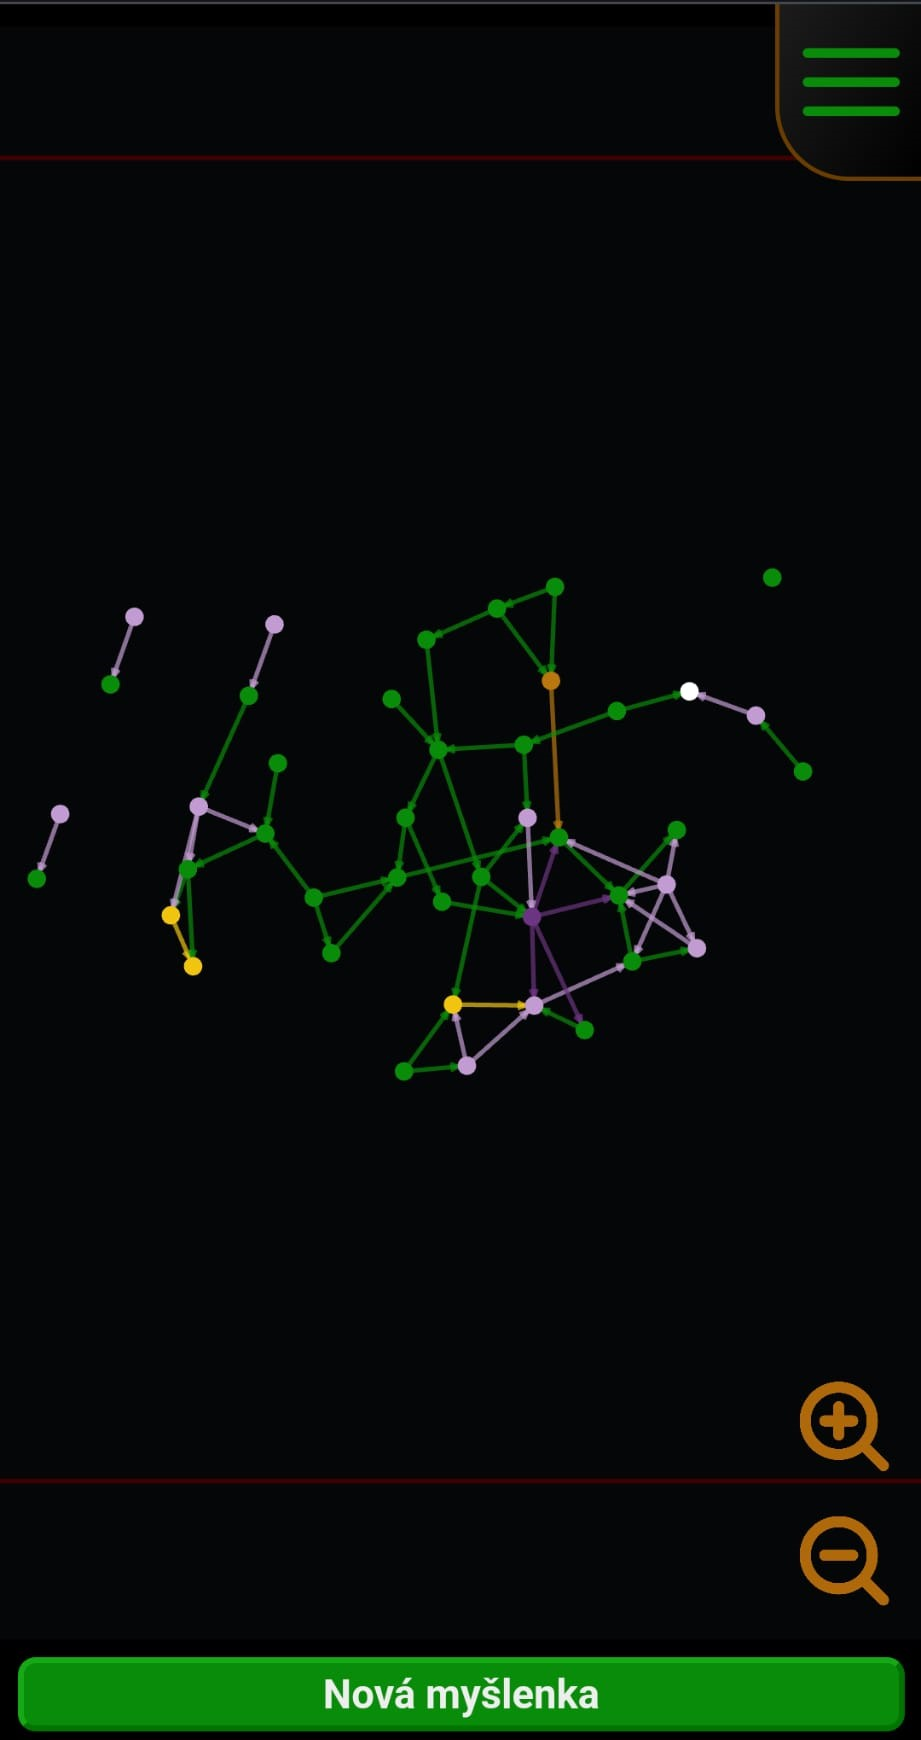
\includegraphics[width=100mm, keepaspectratio]{img/afantazie_first_stage_done.jpg}
    \caption{Aphantasia graph view at the end of the small graph development stage}
    \label{obr:afantazie_selfie}
\end{figure}

\begin{figure}[p]\centering
    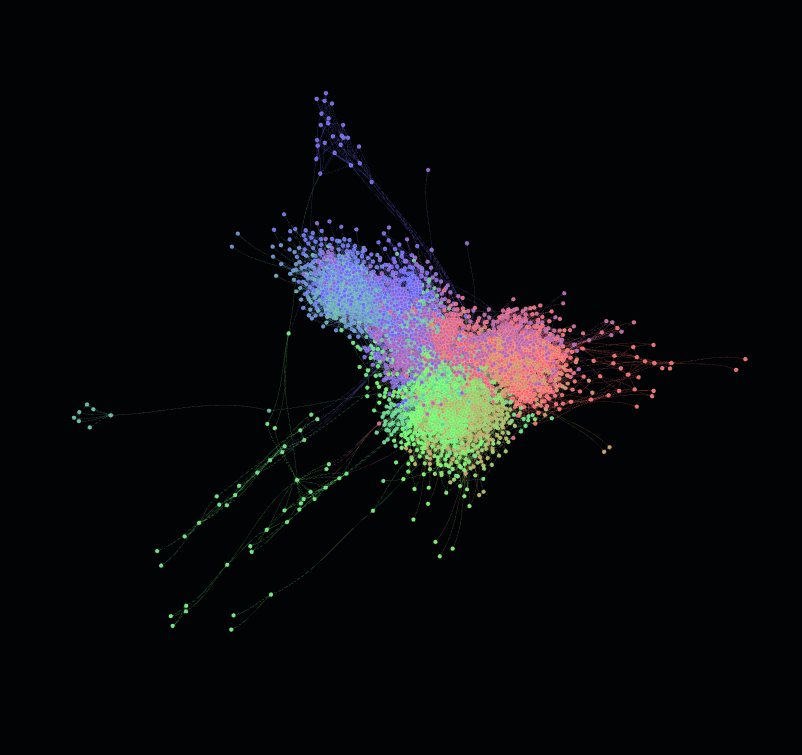
\includegraphics[width=140mm, keepaspectratio]{img/Afantazie_cithep_3000.png}
    \caption{The first 3000 nodes of the CitHep dataset visualized in Aphantasia (before big graph solution)}
    \label{obr:afantazie_cithep_3k}
\end{figure}

\subsection{FDL Implementation}

The core of our FDL implementation is a set of two forces - pull and push.
These forces are defined as functions accepting distance between the nodes and returning a force that should be applied to them.

These functions are defined in the graphParameters.ts file and currently look like this:
\begin{lstlisting}
export const pullForce = (borderDist: number) => {
    if (borderDist <= 0) {
        return borderDist;
    }
    const computed = 0.01 *
        (borderDist - IDEAL_LINKED_DISTANCE);
    const limited = computed > MAX_PULL_FORCE
        ? MAX_PULL_FORCE
        : computed < -MAX_PULL_FORCE
            ? -MAX_PULL_FORCE
            : computed;

    const final = Math.sign(limited) === -1
        ? limited / EDGE_COMPRESSIBILITY_FACTOR
        : limited;

    return final;
};
export const pushForce = (borderDist: number) => {
    if (borderDist === 0) {
        return 0;
    }
    if (borderDist < 0) {
        return -borderDist;
    }
    const computed = 5 / Math.sqrt(borderDist);
    return Math.min(MAX_PUSH_FORCE, computed);
};
\end{lstlisting}

Note that the pull force can be negative. This is intentional as the connected nodes should be attracted not towards each other but towards a certain ideal edge distance.
This distance is parameterized as IDEAL\_LINKED\_DISTANCE.

The numbers inside the functions are the respective force strength parameters.

\subsection{Parametrization}
As stated in Section \ref{sec:force_directed_layout}, the FDL algorithm is highly dependent on the parameters set by the user.
Thus, as expected, we had to implement and configure number of parameters in order to make the graph view a smooth and enjoyable experience.
The full list of parameters we implemented can be found in Administrator documentation in Chapter \ref{sec:graph_layout_parameterssec:graph_layout_parameters}.

Here, we will discuss what led us to implement many of these parameters - jitter.
In some situations, particularly when the graph was not yet fully stabilized, and there were a larger amount of nodes in a small area,
the nodes had the tendency to oscillate quickly.

Parametrizing the forces themselves helped a little but not enought to mitigate the issue.
Instead we implemented a momentum system, where the nodes would not react to the forces immediately but would instead gradually accelerate based on forces applied.
The momentum system is influenced by dampening system - a set of parameters controlling how much the forces applied to the momentum and the momentum itself are reduced each frame.

The jitter was not completely eliminated but was reduced to a level where it was not noticeable in normal use.
We also believe that if the problem arises again, we will be able to alter the parameters accordingly and reduce the problem further.

\section{Big Graph Visualization}
\label{sec:big_graph_implementation}

In the final stage of the development, we implemented the big graph solution.

\subsection*{State management}

So far, we used React states and contexts to hold and manage the the graph context.
This worked for a simple small graph approach, but we were not happy with this approach once the context started to become more complicated
as we had little control over the state from the PixiJS code.

A solution we used is a react library called Zustand \cite{zustand_homepage}.
This library allows minimal state management in React that is compatible with external (meaning non-React) code.

\subsection*{Dynamic loading}
At the beginning of the development, we used one endpoint for all the data at once.
That worked until around 500 thoughts, after which the loading time started to become noticeable. 

The obvious solution was to load only a subset of the data at a time. We implemented this idea in two ways:
\begin{itemize}
    \item \textbf{Temporal API endpoints} - Client requests a new subset of nodes in the form of "beforeId / afterId / aroundId".
 Thanks to the ascending ID increment approach, it translates to the chronological order of the nodes.
 When the time window exceeds the currently loaded data, it gets updated with missing nodes from the relative past or future.
    \item \textbf{Neighborhood API endpoints} - Breadth-first search starting in a given node up to a given depth is used to implement graph exploration.
\end{itemize}

This approach worked not just as an optimization technique but we ended up building our big graph handling on it.
In Figure \ref{obr:afantazie_action_flow}, we can see the logic flow of the big graph rendering solution.
Aphantasia uses two arrays of rendered thoughts - temporal array and neighborhood array.

To keep track of which thoughts should be visible on screen as well as fetching and updating temporal and neighborhood thoughts,
we created the file thoughtsProvider.ts.

\begin{figure}[h]\centering
    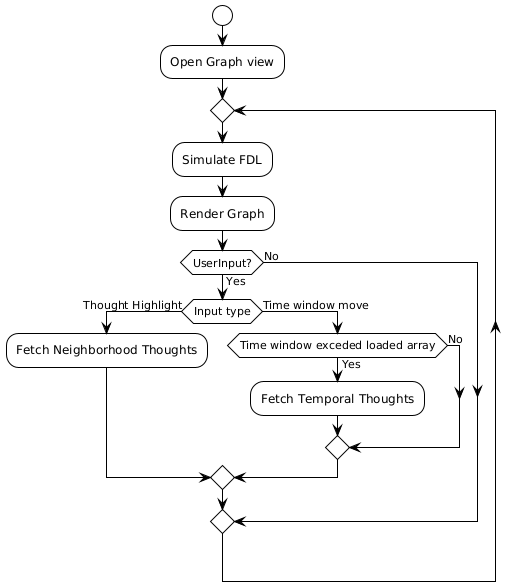
\includegraphics[width=100mm, keepaspectratio]{img/afantazie_graph_view_flow.png}
    \caption{The logic flow of the big graph rendering solution}
    \label{obr:afantazie_action_flow}
\end{figure}

\subsection{Frontend Architecture}
\label{sec:frontend_architecture}

The frontend architecture is much less clear-cut than the backend
but we visualized the relationship between the main source code files in Figure
\ref{obr:afantazie_frontend_architecture}.
All of the graph-related code sits inside the src/pages/graph directory of the AfantazieWeb project
and the containers in the diagram correspond to the folder structure.

\begin{figure}[p]\centering
    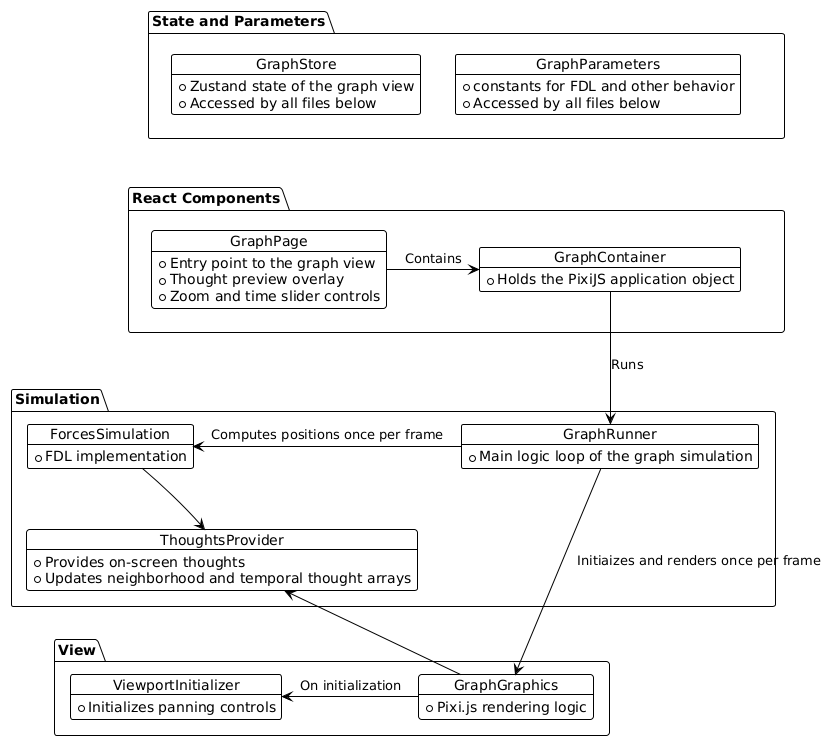
\includegraphics[width=140mm, keepaspectratio]{img/afantazie_frontend_architecture.png}
    \caption{The frontend architecture of Aphantasia}
    \label{obr:afantazie_frontend_architecture}
\end{figure}

Let us look at the individual parts of the frontend architecture:
\subsubsection*{React}
\textbf{Graph Page} contains the UI elements of the graph view:
\begin{itemize}
    \item Content preview
    \item Controls (zoom and time slider)
    \item Time window date label
    \item New thought button
\end{itemize}
It also handles much of the initialization logic, such as getting the thought ID from the URL and fetching the appropriate data
(either the latest or around the requested thought).

\textbf{Graph Container}
This component is the bridge between React and PixiJS code. It calls the run() method of the \textbf{Graph Runer}.

\subsection*{Simulation}
In the Simulation directory, we find three files:
\begin{itemize}
    \item \textbf{Graph Runner} - Contains the main logic loop of the graph simulation.
 Its run() method is called by the Graph Container, and it initializes the graphics,
 runs the render function and the simulation functions.
    \item \textbf{Forces Simulation} - Custom FDA implementation.
    \item \textbf{ThoughtsProvider} - Responsible for providing the temporal and neighborhood thoughts as well as
 fetching data from the backend based on time window position and graph exploration state.
\end{itemize}

The source code of the main logic loop of the application (located in the file graphRunner.ts) is shown below.
Note that the code is simplified for the sake of brevity.

% \begin{minipage}{\linewidth}
\begin{lstlisting}
export default function runGraph(app: Application) {
    const renderGraph = initGraphics(app);
    useGraphStore.getState().setFrame(0);

    // main application loop
    app.ticker.add((_) => {
        const graphState = useGraphStore.getState();

        // cache thoughts
        if (graphState.frame === THOUGHTS_CACHE_FRAME) {
            ...
            localStorage.setItem('thoughts-cache',
                JSON.stringify(thoughtsCache));
        }
            
        // Update temporal thoughts if needed
        updateTemporalThoughts();

        // FDL simulation
        const frame = graphState.frame;
        if (frame < SIMULATION_FRAMES) {
            simulate_one_frame();   
        }
        graphState.setFrame(frame + 1);

        // render the graph
        renderGraph();
    });
}
\end{lstlisting}
% \end{minipage}

\subsection*{Graphics}
This directory contains two files:
\begin{itemize}
    \item \textbf{Graphics} - Contains the initializeGraphics() method which returns a callback function render()
 called by the Graph Runner every loop.
    \item \textbf{ViewportInitializer} - Contains the addDraggableViewport() method
 which sets up the viewport for the graph. 
\end{itemize}

\subsection*{State and parameters}
Here we find two files:
\begin{itemize}
    \item \textbf{Graph Store} - Zustand store for the graph state.
    \item \textbf{Graph Parameters} - Constants used in the graph view, \gls{FDL} and other behavior.
\end{itemize}

\section{Final List of Features}
This section provides a deeper look into the user-facing features and technical aspects of the application.
More user-focused documentation will be available in Chapter \ref{chap:user_documentation}.

\subsection{AuthX/Y}
The application includes user account functionality supporting authentication and authorization.
Users can register, log in, and log out. Most pages and features are accessible only to logged-in users.

Passwords are hashed using \gls{sha256} encryption and must meet minimal requirements:
\begin{itemize}
\item At least eight characters
\item At least one uppercase letter
\item At least one lowercase letter
\item At least one number
\end{itemize}

Login is managed via \gls{jwt} stored in \gls{local_storage}.
Tokens expire after one day, and a refresh token mechanism is not implemented, requiring users to re-login every 24 hours.

Tokens are currently sent in URL parameters for SignalR WebSocket connections.
This practice is not ideal and should be replaced in the future.
A possible solution involves a ticketing system where a logged-in client would request a ticket from the API.
This ticket would then authorize the WebSocket connection, avoiding token exposure in the URL. %\xxx{cit?}

\subsection{Pages}
Thanks to React, the graph view is one of many pages in the application. There are currently ten pages:
\begin{itemize}
\item \textbf{Homepage}: Displays a feed of recent thoughts and navigation buttons (Figure \ref{obr:afantazie_welcome_and_homepage})
\item \textbf{Welcome Page}: Similar to the homepage but tailored for unregistered users (Figure \ref{obr:afantazie_welcome_and_homepage})
\item \textbf{About Page}: Provides information about the project
\item \textbf{Chat Room}: A basic real-time chat
\item \textbf{Settings Page}: Contains user settings and a logout button
\item \textbf{Login and Registration Pages}
\item \textbf{Notifications Page}: Displays replies from other users
\item \textbf{Graph View}: Enables users to view thoughts
\item \textbf{Thought Creation Page}: Allows users to create new thoughts
\end{itemize}

\begin{figure}[p]
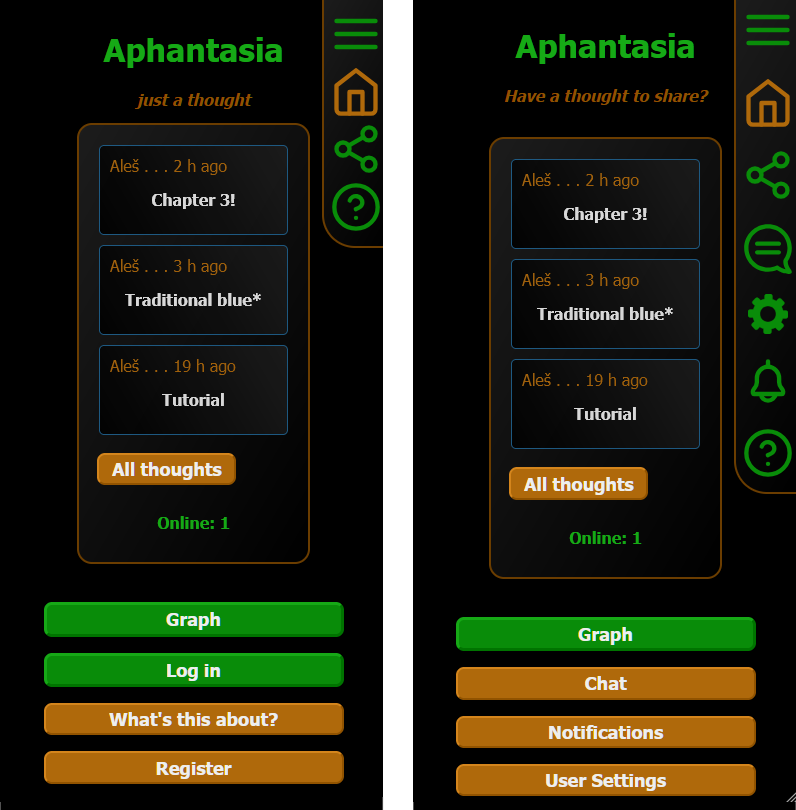
\includegraphics[width=130mm, keepaspectratio]{img/afantazie_welcome_and_home_page.png}
\caption{The Welcome page and homepage of Aphantasia}
\label{obr:afantazie_welcome_and_homepage}
\end{figure}

\subsection{Localization}
Initially, we developed a Czech version of the application and later added an English version.
For frontend \gls{localization}, we utilized two JSON files and a Localization object which returns 
either Czech or English text based on \gls{vite} configuration.
This makes the application easily extensible to more languages.

Backend localization was also required, as the API returns localized authentication and validation messages.
To achieve this, we created a Localization project with classes implementing localization interfaces.
During bootstrapping, a specific localization is registered based on configuration. 
While this approach is somewhat cumbersome, it suffices for the limited localization needs of the backend.

\subsection{Custom Graph Rendering Engine}

The graph view is the primary feature of Aphantasia and the most complex part of the application.
Its basic features include:
\begin{itemize}
\item \textbf{Zooming and Panning}
\item \textbf{Dragging Thoughts}
\item \textbf{Floating Text Titles} (Figure \ref{obr:afantazie_floating_titles})
\item \textbf{Thought Highlighting} (On Figure \ref{obr:afantazie_mobile_graph_view} and \ref{obr:afantazie_floating_titles})
\end{itemize}

\begin{figure}[p]
    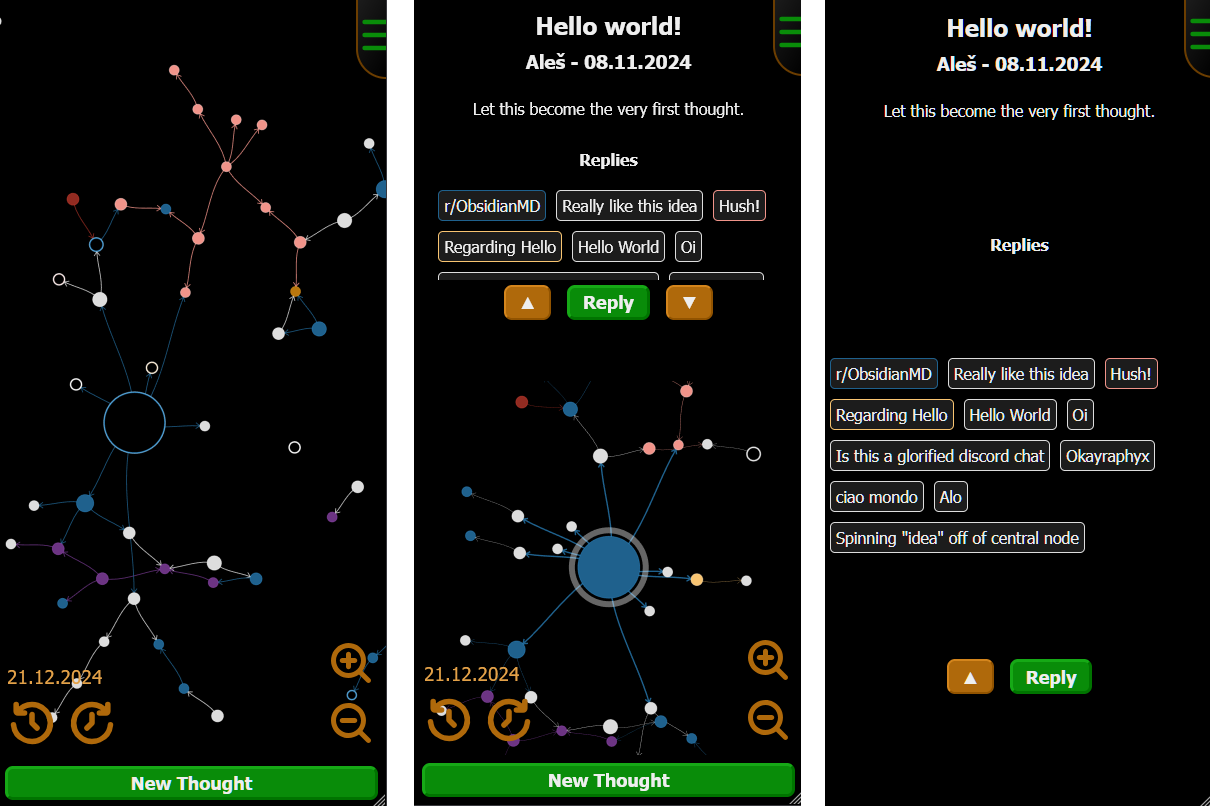
\includegraphics[width=130mm, keepaspectratio]{img/afantazie_mobile_graph_view.png}
    \caption{The graph view on a mobile device - non-highlighted mode, half-screen preview, and fullscreen preview, respectively}
    \label{obr:afantazie_mobile_graph_view}
\end{figure}

\begin{figure}[p]
    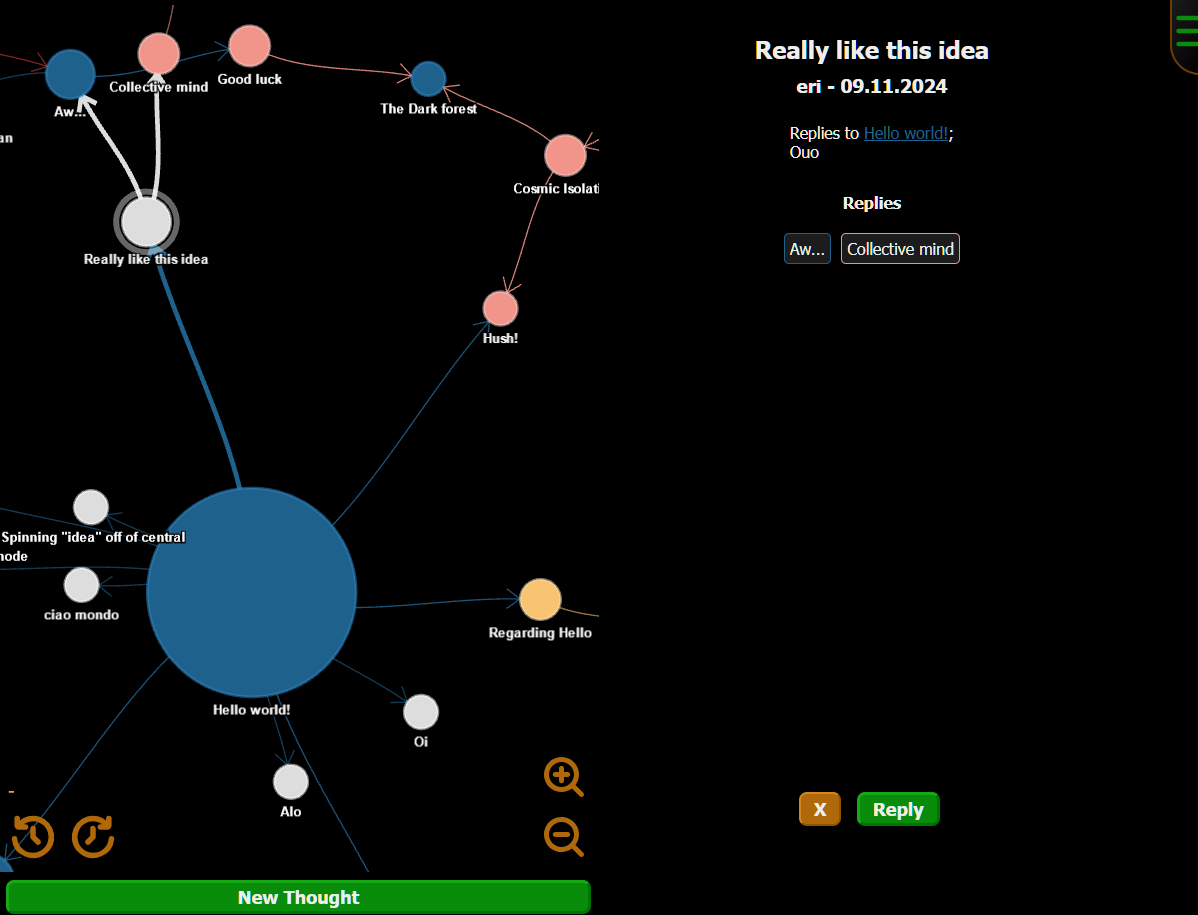
\includegraphics[width=130mm, keepaspectratio]{img/afantazie_floating_titles.png}
    \caption{Floating titles in the graph view on desktop}
    \label{obr:afantazie_floating_titles}
\end{figure}

\begin{figure}[p]
    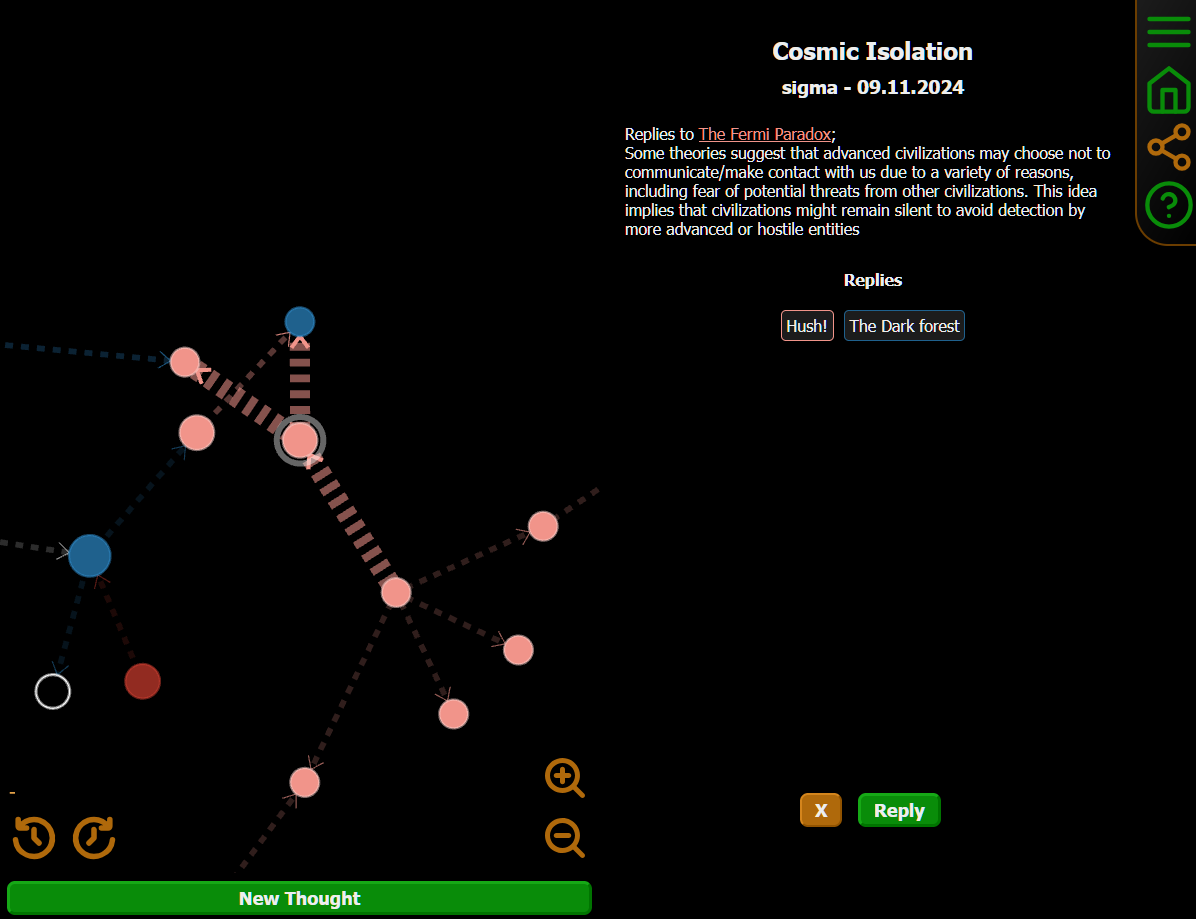
\includegraphics[width=130mm, keepaspectratio]{img/afantazie_animated_edges.png}
    \caption{Animated edges in the graph view}
    \label{obr:afantazie_animated_edges}
\end{figure}

\subsubsection*{On-screen Thoughts Limit}
The On-screen thoughts limit is a critical part of our big graph rendering solution.
The default value is 100, but users can adjust it in the settings.

The idea behind it is to always render, at most, this number of thoughts on screen.
And to view more user input is required - either by moving the time slider or by using the graph exploration feature, both of which we will talk about briefly.

The limit is demonstrated in Figure \ref{obr:afantazie_production_dataset_in_time_window} and \ref{obr:afantzazie_production_dataset_640_nodes} with the values set to 300 and 700, respectively.

\subsubsection*{Time Slider}
Combining the On-screen thoughts limit, dynamic loading, and two UI buttons resulted in a feature we call the Time slider.
It allows users to move a conceptual time window smoothly into the past or future by holding the corresponding button.
The resulting layout using the time slider is demonstrated in Figure \ref{obr:afantazie_production_dataset_in_time_window}
with 641 thoughts on afantazie.cz viewed in three different time windows of length 300.

Above the time slider controls, there is a label showing the current time window's position - the creation date of the newest thought on the screen.
The label can be seen in the bottom left in Figure \ref{obr:afantazie_mobile_graph_view}.

New thoughts appear either in their cached positions (see Layout caching section below) or in a circular pattern around the simulation container's center.
When not yet cached, the appearance of newer/older nodes creates a visually appealing effect as the thoughts gradually appear in what resembles a loading spinner.

\subsubsection*{Live Preview}
When the time slider moves beyond the last thought, the application enters live preview mode indicated by 'Now...' apearing in place of the time window's date in bottom left.
In this mode, the client listens to new thoughts and adds them to the graph in real-time.

While this feature enhances interactivity, it has only been tested with two users creating thoughts simultaneously.
Higher activity levels could potentially overwhelm the system, but until there is an active user base, this remains
a theoretical concern.

We implemented this feature using long polling, meaning that the client periodically sends
requests to the server to check for new thoughts. This approach is a bit wasteful, especially considering that we already have an active
signalR connection to use across the entire application.
In the future we will replace long polling with the active signalR connection.

\subsubsection*{Graph Exploration}
The neighborhood API endpoint powers graph exploration demonstrated in Figure \ref{obr:afantazie_mobile_graph_view}.
After clicking on a node, link, or reply, the client loads the neighborhood of the newly highlighted thought, enabling interactive exploration.

In the example and many other screenshots provided in this work, some thoughts appear hollowed out.
This effect triggers when the thought's direct neighbors (links or replies) are not currently rendered on screen, signaling that there is more to explore behind it.
When the neighbors of a node are all visible, the node is filled with its author's color.

Currently, the graph exploration neighborhood array does not respect the on-screen thoughts limit and loads all neighbors of the highlighted thought up to a given depth.
This didn't pose a problem with the datasets we used but could be a significant issue with highly connected datasets.

\subsubsection*{Thoughts Layout Caching}
The browser's local storage caches the thoughts layout after a period of inactivity.
The length of this period is parametrizable by a number of frames,
with the current value set to 1 000 frames, which corresponds to around 30 seconds of inactivity on most devices.
When a thought leaves the screen and later reappears, it retains its previous position.
This feature facilitates graph stability during time sliding and between sessions and removes the need for the graph to stabilize again and again.

Paired with the time slider, this approach produced an unexpected emergent behavior. As the \gls{production} dataset grew beyond 500 thoughts (five times the default on-screen limit), it remained possible to create a stabilized graph across the entire dataset.
Moving the time slider across such a stabilized layout is a uniquely satisfying experience, which we believe sets Aphantasia apart.
To some extent, this feature is visible in Figure \ref{obr:afantazie_production_dataset_in_time_window} but it is best experienced in the live application.

The cache currently has no size limit and is not cleared automatically, which could be a potential issue with big datasets and longer graph view sessions.
Logged-in users can, however, delete cached positions in settings to force the graph to re-stabilize.

\begin{figure}[p]
    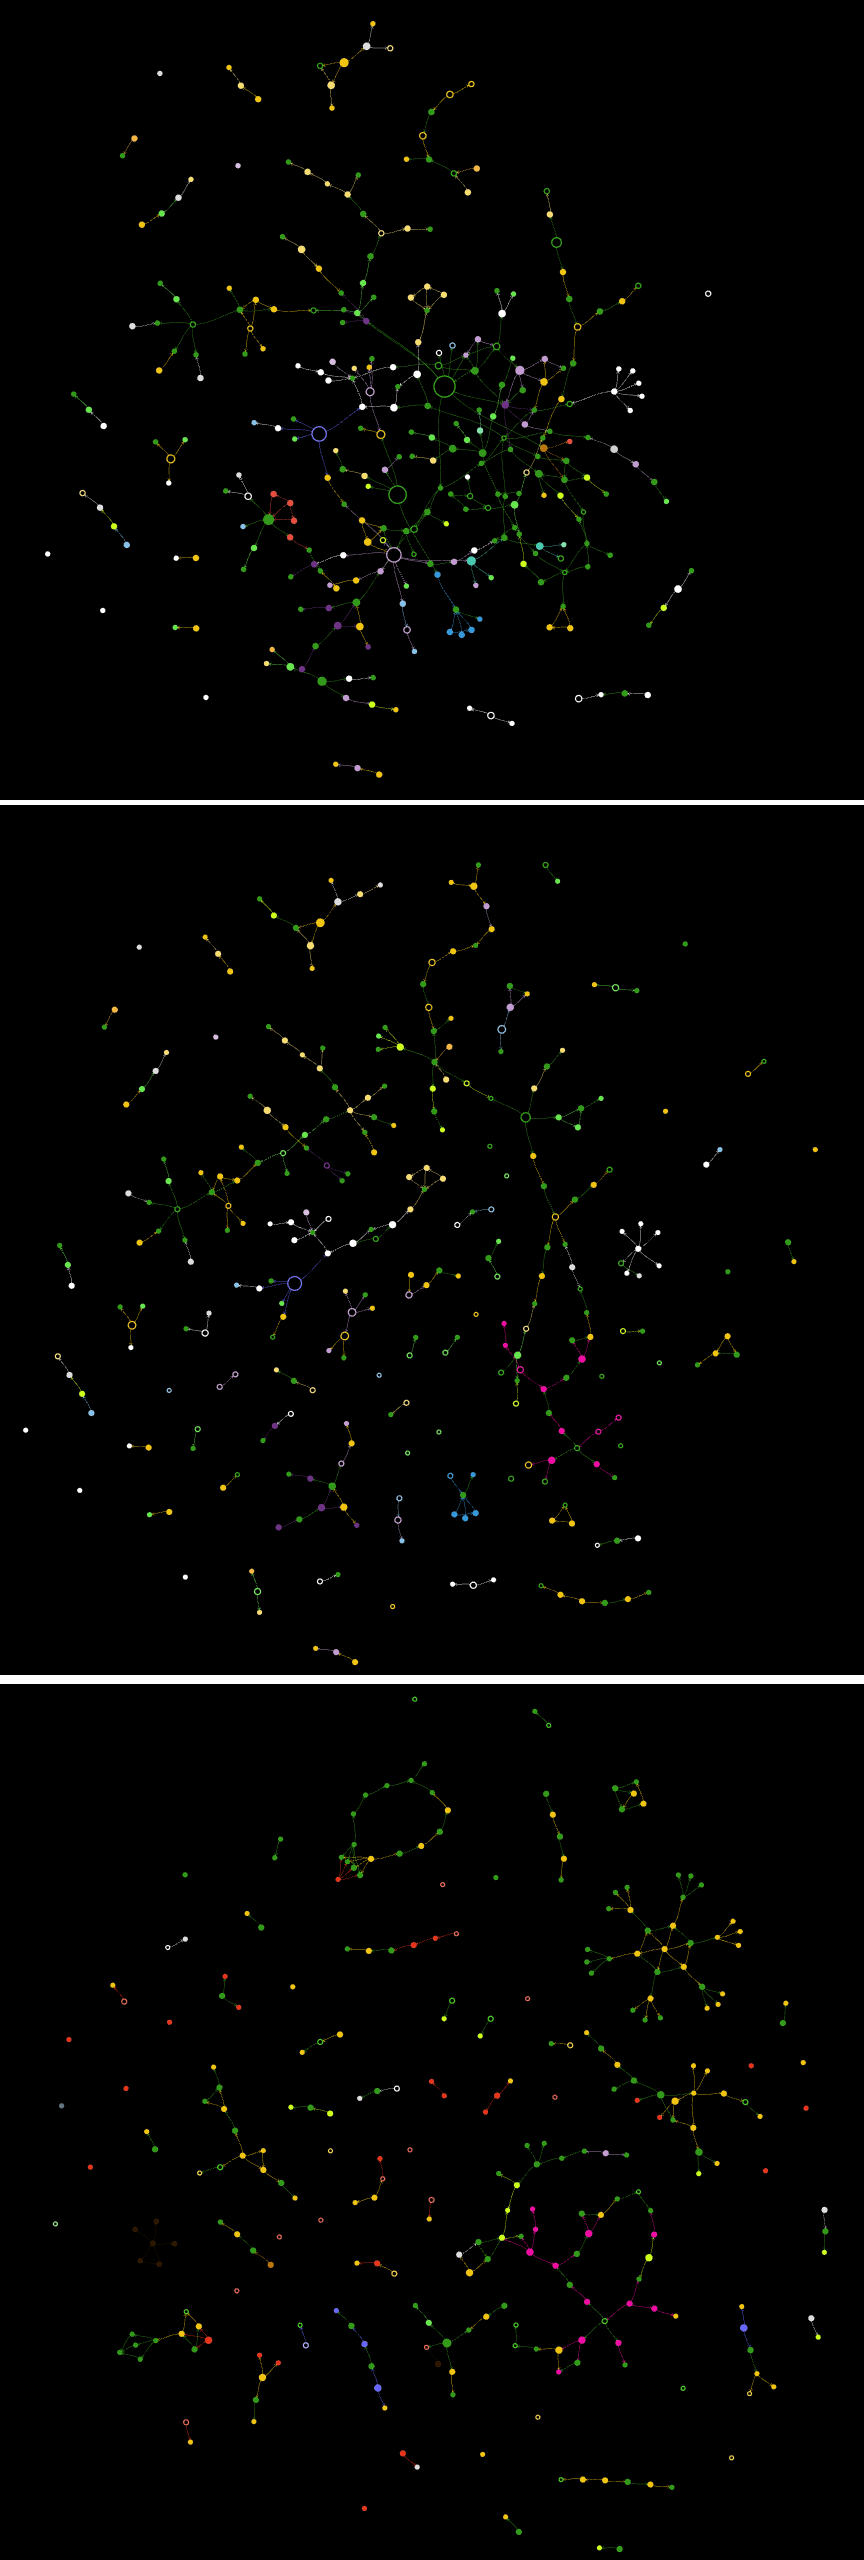
\includegraphics[height=200mm, keepaspectratio]{img/afantazie_production_dataset_in_time_window.png}
    \caption{Aphantasia with the Czech production dataset in stabilized temporal layout (641 nodes in three time windows of length 300)}
    \label{obr:afantazie_production_dataset_in_time_window}
\end{figure}

\begin{figure}[p]
    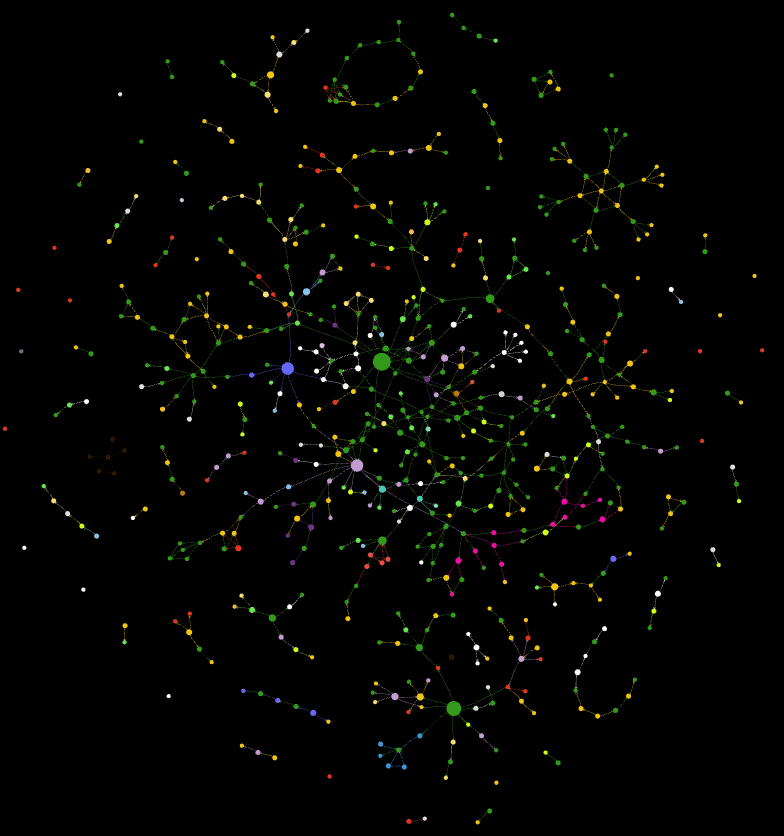
\includegraphics[width=130mm, keepaspectratio]{img/afantzazie_production_dataset_641_nodes.png}
    \caption{The entire dataset of afantazie.cz (641 nodes) in a single time window}
    \label{obr:afantzazie_production_dataset_640_nodes}
\end{figure}


\chapter{The Completed Application}

As of the time of writing, Aphantasia is a functional proof of concept with a simple UI, graph view, and several rudimentary features.
While there are bugs to resolve and features to add, the application is usable and publicly accessible.

We are hosting two public instances:
\begin{itemize}
\item English version at \href{https://aphantasia.io}{aphantasia.io}
\item Czech version at \href{https://afantazie.cz}{afantazie.cz}
\end{itemize}

\section{Features}
This section provides a deeper look into the user-facing features and technical aspects of the application.
More user-focused documentation will be available in Chapter 6.

\subsection{AuthX/Y}
The application includes user account functionality, supporting authentication and authorization.
Users can register, log in, and log out. Most pages and features are accessible only to logged-in users.

Passwords are hashed using \gls{sha256} encryption and must meet minimal requirements:
\begin{itemize}
\item At least 8 characters
\item At least one uppercase letter
\item At least one lowercase letter
\item At least one number
\end{itemize}

Login is managed via \gls{jwt} stored in \gls{local_storage}.
Tokens expire after one day, and a refresh token mechanism is not implemented, requiring users to re-login every 24 hours.

Tokens are currently sent in URL parameters for SignalR WebSocket connections.
This practice is not ideal and should be replaced in the future.
A possible solution involves a ticketing system where a logged-in client would request a ticket from the API.
This ticket would then authorize the WebSocket connection, avoiding token exposure in the URL. %\xxx{cit?}

\subsection{Pages}
Thanks to React, the graph view is one of many pages in the application. There are currently ten pages:
\begin{itemize}
\item \textbf{Homepage}: Displays a feed of recent thoughts and navigation buttons (Figure \ref{obr:afantazie_welcome_and_homepage})
\item \textbf{Welcome Page}: Similar to the homepage but tailored for unregistered users (Figure \ref{obr:afantazie_welcome_and_homepage})
\item \textbf{About Page}: Provides information about the project
\item \textbf{Chat Room}: A basic real-time chat
\item \textbf{Settings Page}: Contains user settings and a logout button
\item \textbf{Login and Registration Pages}
\item \textbf{Notifications Page}: Displays replies from other users
\item \textbf{Graph View}: Enables users to view thoughts
\item \textbf{Thought Creation Page}: Allows users to create new thoughts
\end{itemize}

\begin{figure}[p]
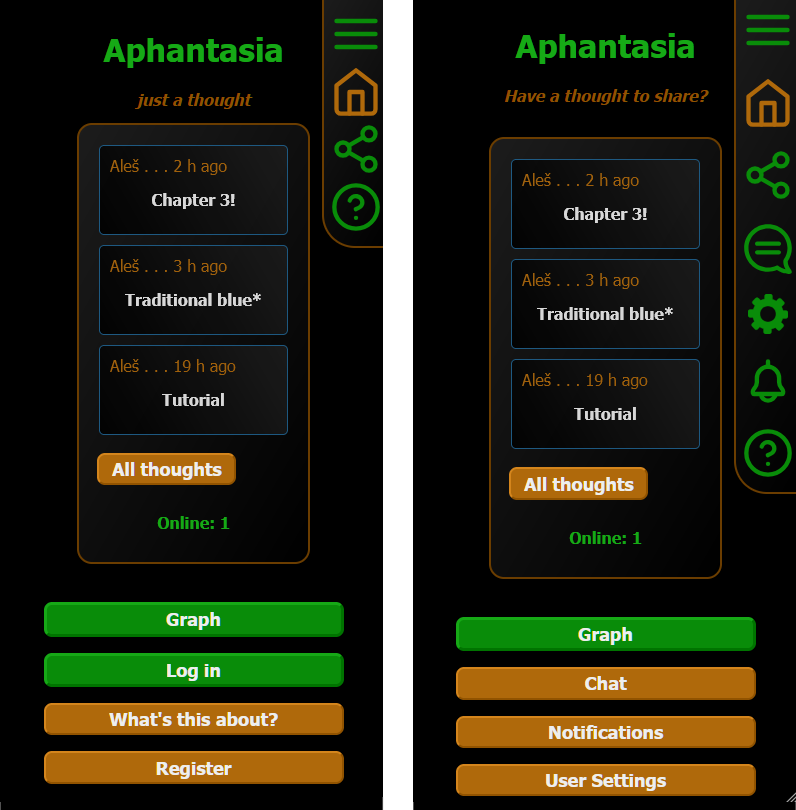
\includegraphics[width=130mm, keepaspectratio]{img/afantazie_welcome_and_home_page.png}
\caption{The Welcome page and homepage of Aphantasia}
\label{obr:afantazie_welcome_and_homepage}
\end{figure}

\subsection{Localization}
Initially, we developed a Czech version of the application and later added an English version.
For frontend \gls{localization}, we utilized two JSON files and a Localization object which returns 
either czech or english text based on \gls{vite} configuration.
This makes the application easily extensible to more languages.

Backend localization was also required, as the API returns localized authentication and validation messages.
To achieve this, we created a Localization project with classes implementing localization interfaces.
During boostrapping a specific localization is registered based on configuration. 
While this approach is somewhat cumbersome, it suffices for the limited localization needs of the backend.

\subsection{Custom Graph Rendering Engine}

The graph view is the primary feature of Aphantasia and the most complex part of the application.
Its basic features include:
\begin{itemize}
\item \textbf{Zooming and Panning}
\item \textbf{Dragging Thoughts}
\item \textbf{Floating Text Titles} (figure \ref{obr:afantazie_floating_titles})
\item \textbf{Thought Highlighting} (On figures \ref{obr:afantazie_mobile_graph_view} and \ref{obr:afantazie_floating_titles})
\end{itemize}

\begin{figure}[p]
    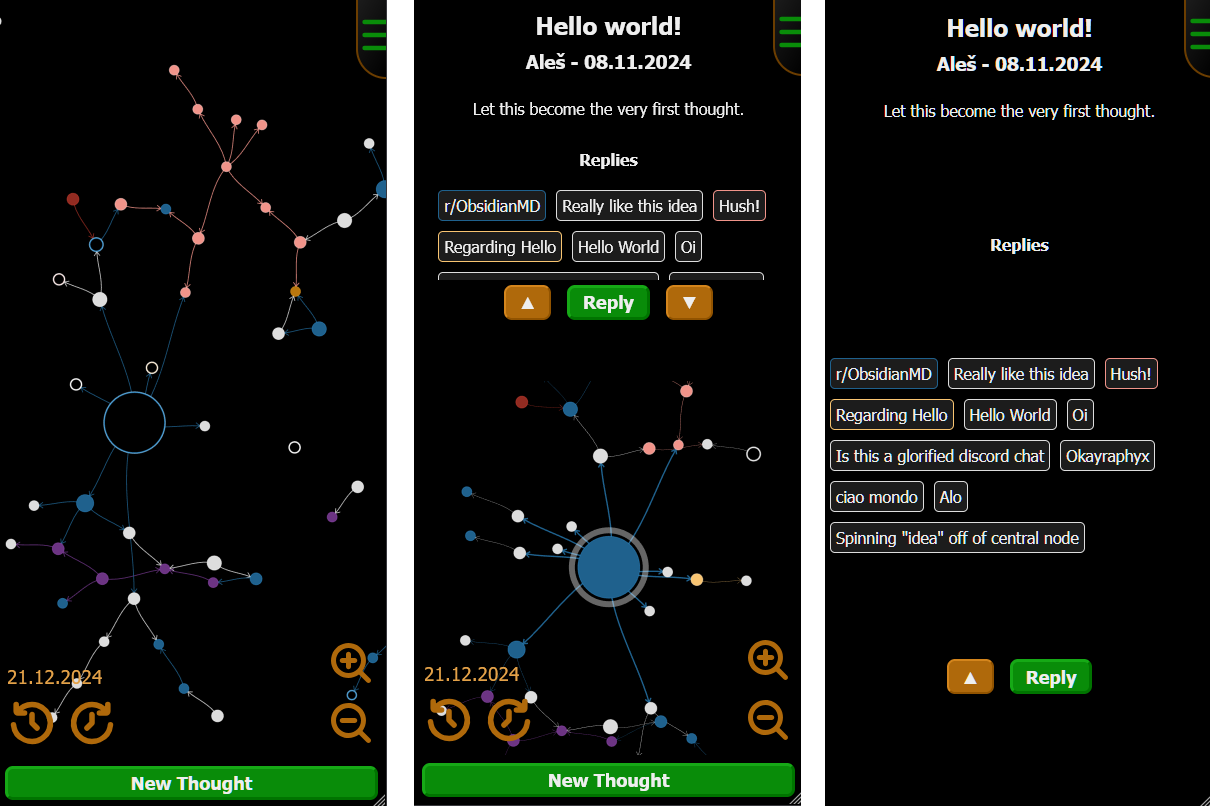
\includegraphics[width=130mm, keepaspectratio]{img/afantazie_mobile_graph_view.png}
    \caption{The graph view on mobile device - non-highlighted mode, half-screen preview and fullscreen preview respectively}
    \label{obr:afantazie_mobile_graph_view}
\end{figure}


\begin{figure}[p]
    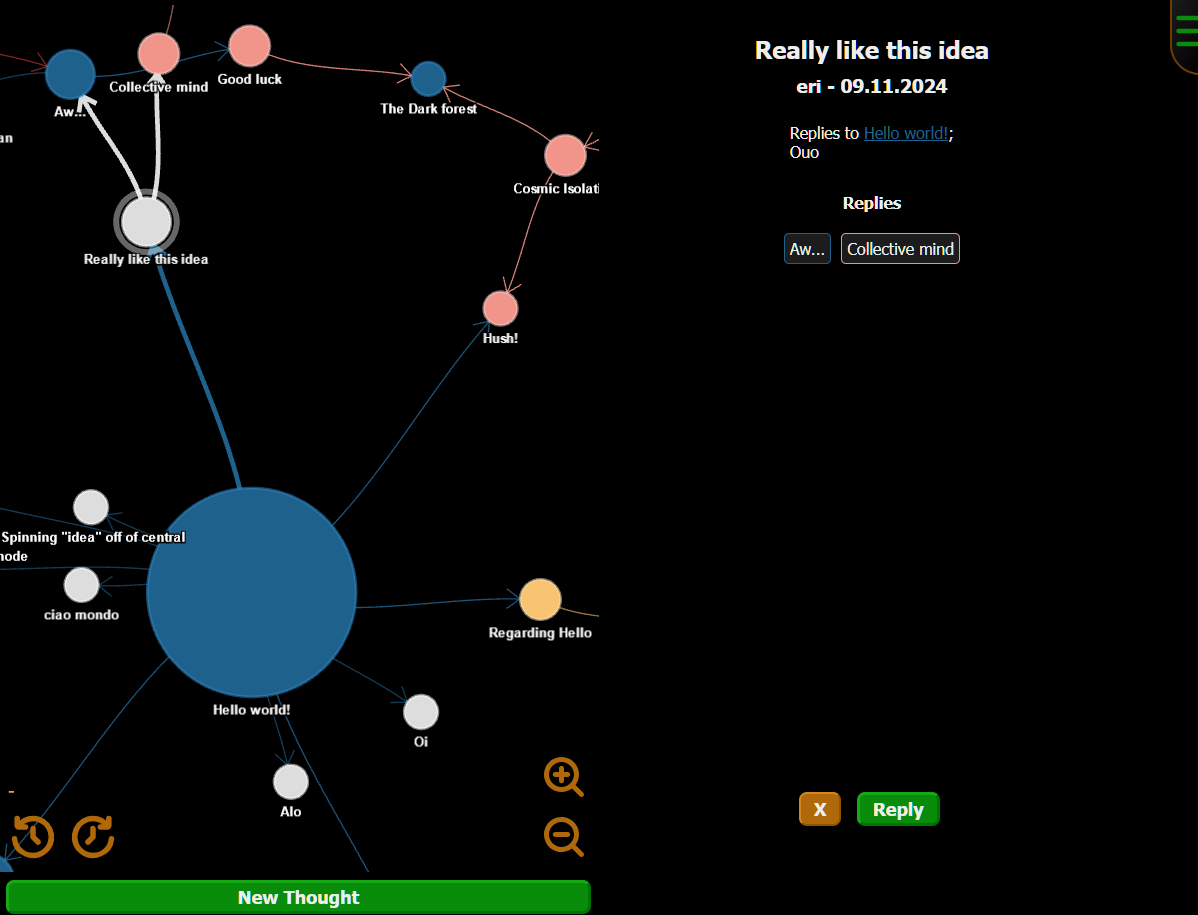
\includegraphics[width=130mm, keepaspectratio]{img/afantazie_floating_titles.png}
    \caption{Floating titles in the graph view on desktop}
    \label{obr:afantazie_floating_titles}
\end{figure}

% The graph view utilizes Pixi.js for rendering, \gls{zustand} for state management, and a custom \gls{FDL} implementation.
% move to implementation- todo

We began with pull and push forces and incrementally introduced a range of parameterizable settings to the computation.
\begin{itemize}
\item \textbf{Forces}: Pull force, push force, and gravity force, including maximum allowed values and distance thresholds
\item \textbf{Link Distance}: Controls the spacing between connected thoughts
\item \textbf{Momentum Dampening Divisor}: Forces acting on thoughts are divided by this number resulting in a smoother less shaky simumeaning lation
\item \textbf{Stage Size}: The size of the simulation container
\item \textbf{Radius Controls}: Base radius, size multiplier (how much larger more-referenced thoughts are) and maximum radius
\item \textbf{Simulation Falloff Time}: Gradually slows down the \gls{GLA} after each user interaction (dragging, or selecting thoughts and time sliding)
\item \textbf{Frames with Overlap}: Allows newly appeared thoughts to overlap for given amount of frames
\item \textbf{Layout Caching Frequency}: Specifies how often the layout is saved to \gls{local_storage}
\item \textbf{Node Mass}: Allows differently sized thoughts to have proportional influence on each other, with maximum and minimum values also parametrized
\item \textbf{Backlinks Count Force Divisor}: Reduces forces acting on highly connected nodes
\item \textbf{Edges Appearance}: Adjusts thickness and color of highlighted and unhighlighted edges (edges leading in or out of the currently highlighted node)
\item \textbf{Frames with Less Influence}: New thoughts start with no influence over the simulation and gradually gain it over time
\end{itemize}

This is a non-exhaustive list and there are many more parameters controlling the simulation and rendering process.

\begin{figure}[p]
    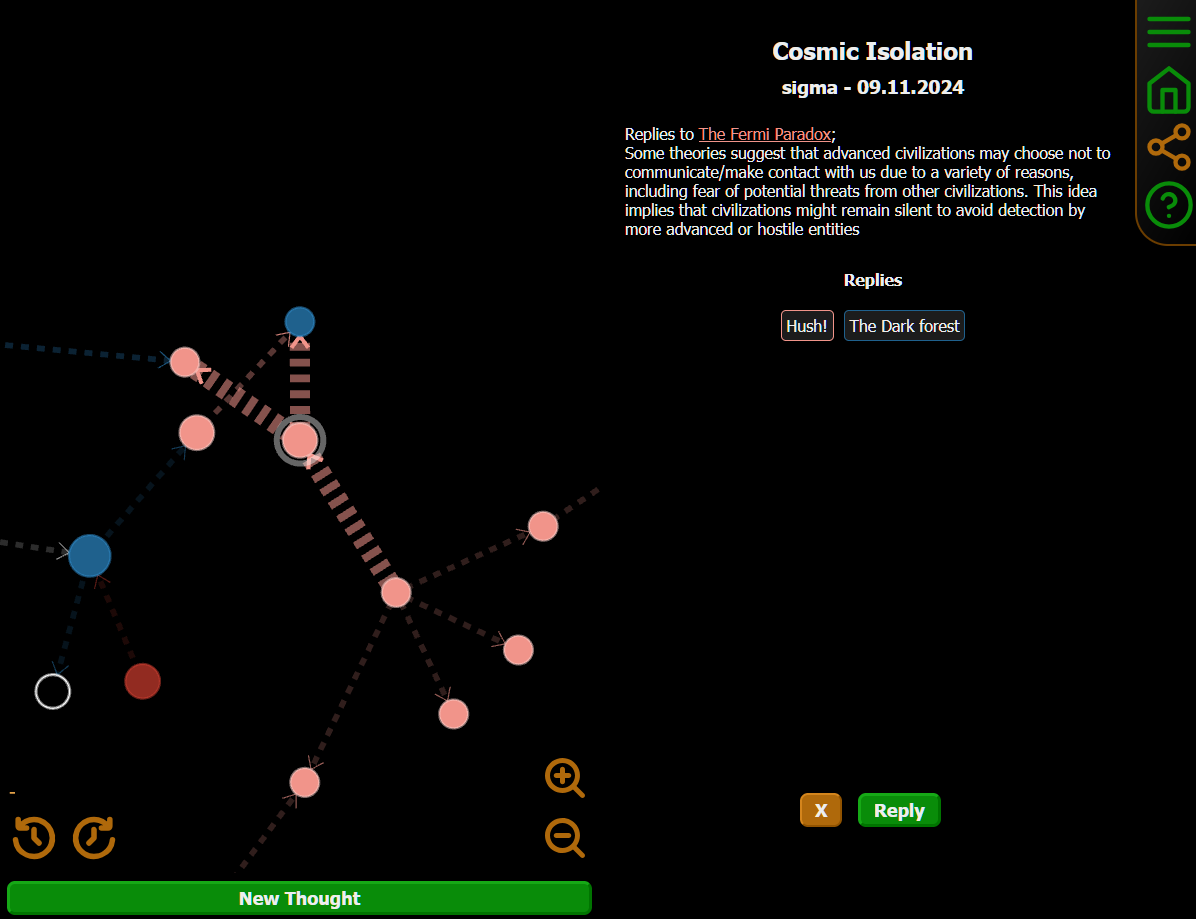
\includegraphics[width=130mm, keepaspectratio]{img/afantazie_animated_edges.png}
    \caption{Animated edges in the graph view}
    \label{obr:afantazie_animated_edges}
\end{figure}
    
\subsubsection*{On-screen thoughts limit}
The On-screen thoughts limit is a critical part of our big graph rendering solution.
The default value is 100, but users can adjust it in the settings.

The idea behind it is to always render at most this number of thoughts on screen.
And to view more user input is required - either by moving the time slider or by using the Graph walk feature, both of which we will talk about briefly.

The limit is demonstrated in figures \ref{obr:afantazie_production_dataset_in_time_window} and \ref{obr:afantzazie_production_dataset_640_nodes} with the values set to 300 and 700 respectively.

\subsubsection*{Time Slider}
Combining the On-screen thoughts limit, dynamic loading, and two UI buttons resulted in a feature we call the Time slider.
It allows users to move a conceptual time window smoothly into the past or future by holding the corresponding button.
The resulting layout using time slider is demonstrated in figure \ref{obr:afantazie_production_dataset_in_time_window}
with 641 thoughts on afantazie.cz viewed in three different time windows of length 300.

Above the time slider controls there is a label showing the current time window's position - the creation date of the newest thought on screen.
You can see the label in bottom left in figure \ref{obr:afantazie_mobile_graph_view}.

New thoughts appear either in their cached positions (see Layout caching section below) or in a circular pattern around the simulation container’s center.
When not yet cached the appearance of newer/older nodes creates a visually appealing effect as the thoughts gradually appear in what resembles a loading spinner.

\subsubsection*{Live Preview}
When the time slider moves beyond the last thought, the application enters live preview mode indicated by 'Now...' apearing in place of the time window's date in bottom left.
In this mode the client listens for new thoughts and adds them to the graph in real time.

While this feature enhances interactivity, it has only been tested with two users creating thoughts simultaneously.
Higher activity levels could potentially overwhelm the interface but until there is an active userbase this remains a theoretical concern.

\subsubsection*{Graph Walk}
The neighborhood API endpoint powers Graph walk demonstrated in figure \ref{obr:afantazie_mobile_graph_view}.
After clicking on a node, link or reply the client loads the neighborhood of the newly highlighted thought, enabling interactive exploration.

In the example as well as many other screenshots provided in this work, some thoughts appear hollowed out.
This effect triggers when thought's direct neighbors (links or replies) are not currently rendered on screen
signalling that there is more to explore behind it.
When the neighbors of a node are all visible, the node is filled with its author's color.

Currently graph walk doesn't respect the on-screen thoughts limit and loads all neighbors of the highlighted thought up to given depth. This didn't pose a problem with the datasets we used but could be a significant issue with highly connected datasets.

\subsubsection*{Thoughts Layout Caching}
The browser’s local storage caches the thoughts layout after a period of inactivity.
The length of this period is parametrizable by number of frames,
with the current value set to 1000 frames which corresponds to around 30 seconds of inactivity on most devices.
When a thought leaves the screen and later reappears, it retains its previous position.
This feature facilitates graph stability during time sliding and between sessions and removes the need for the graph to re-stabilize again and again.

Paired with the Time slider this approach produced an unexpected emergent behavior. As the \gls{production} dataset grew beyond 500 thoughts (five times the default on-screen limit), it remained possible to create a stabilized graph across the entire dataset.
Moving the time slider across such stabilized layout is a uniquely satisfying experience, which we believe sets Aphantasia apart.
To some extent, this feature is visible in figure \ref{obr:afantazie_production_dataset_in_time_window} but it is best experienced in the live application.

The cache currently has no size limit and is not cleared automatically, which could be a potential issue with big datasets and longer graph view sessions.
Logged in users can however delete cached positions in settings to force the graph to re-stabilize.

\begin{figure}[p]
    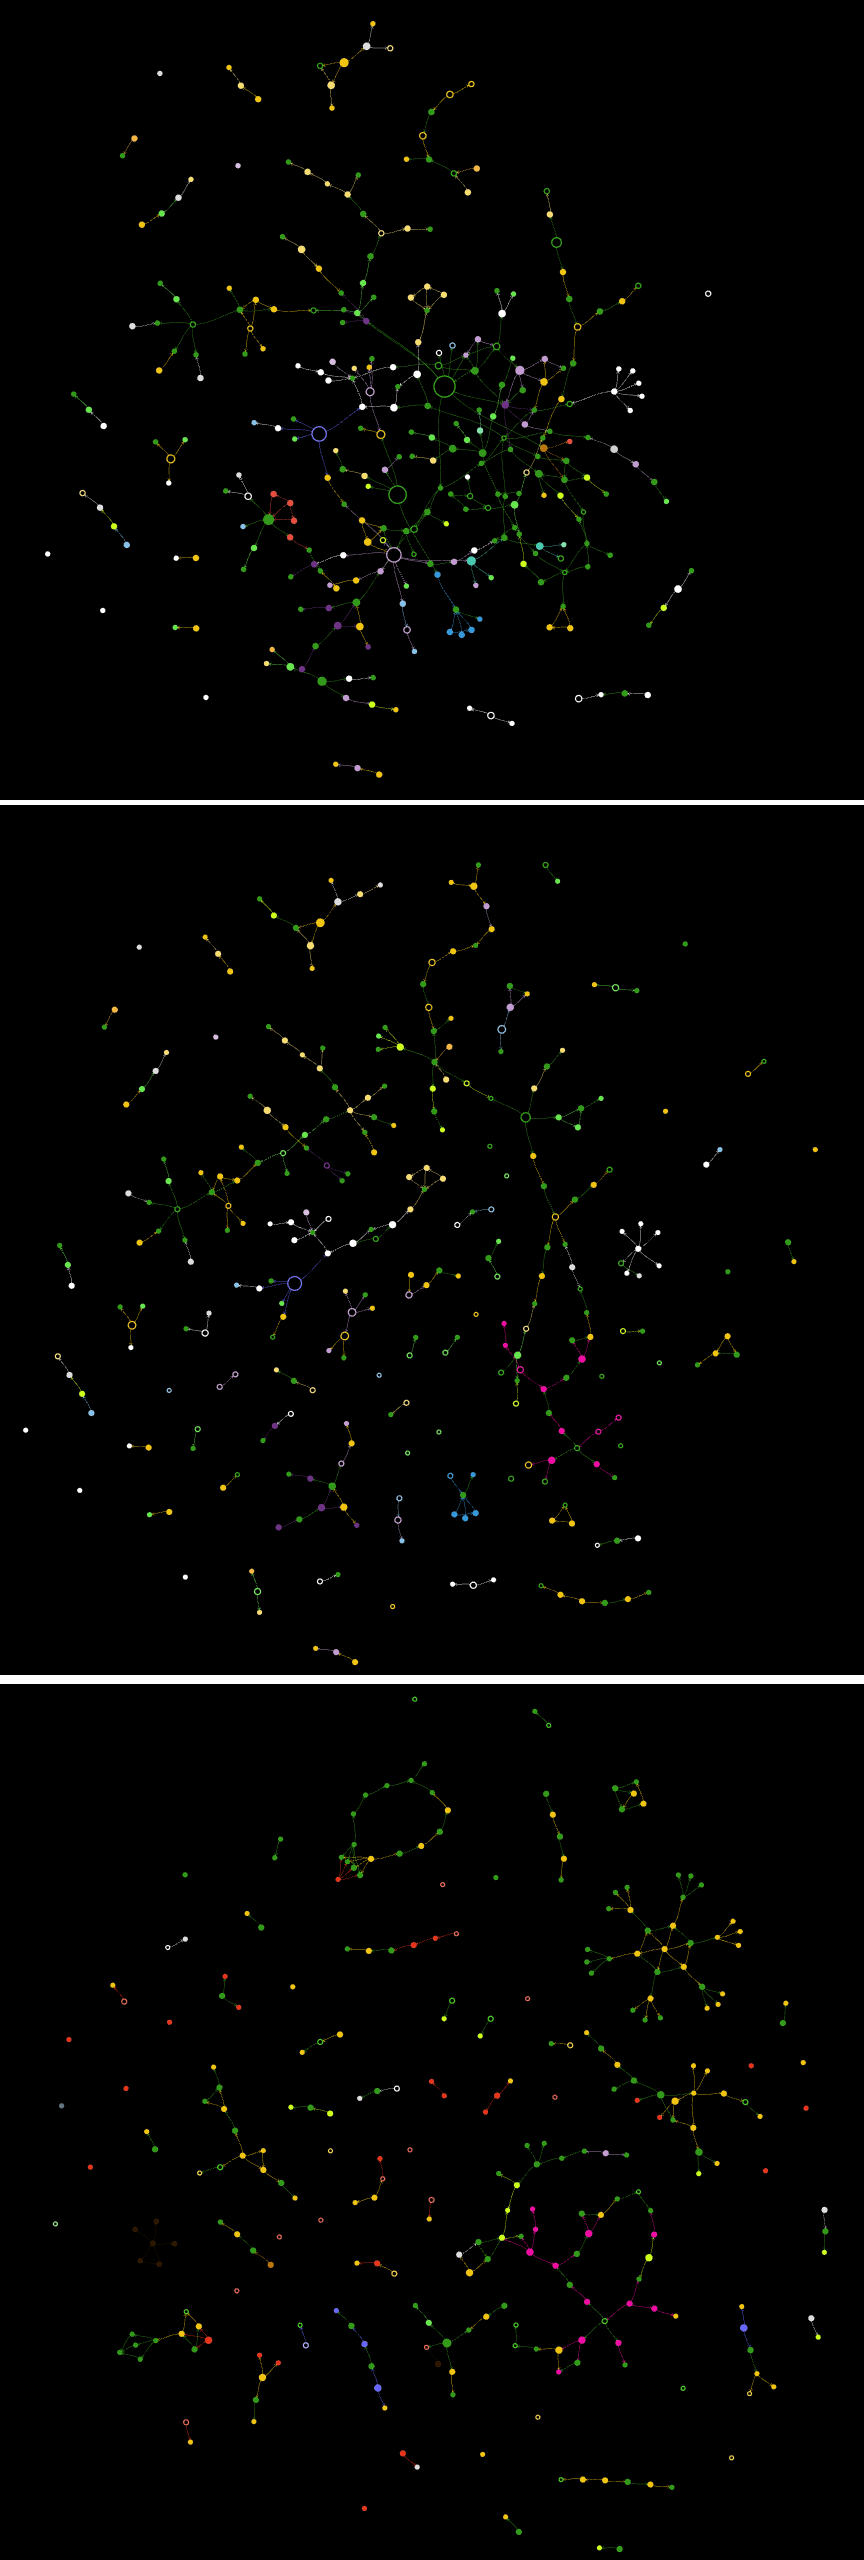
\includegraphics[height=200mm, keepaspectratio]{img/afantazie_production_dataset_in_time_window.png}
    \caption{Aphantasia with the czech production dataset in stabilized temporal layout (641 nodes in three time windows of length 300)}
    \label{obr:afantazie_production_dataset_in_time_window}
\end{figure}

\begin{figure}[p]
    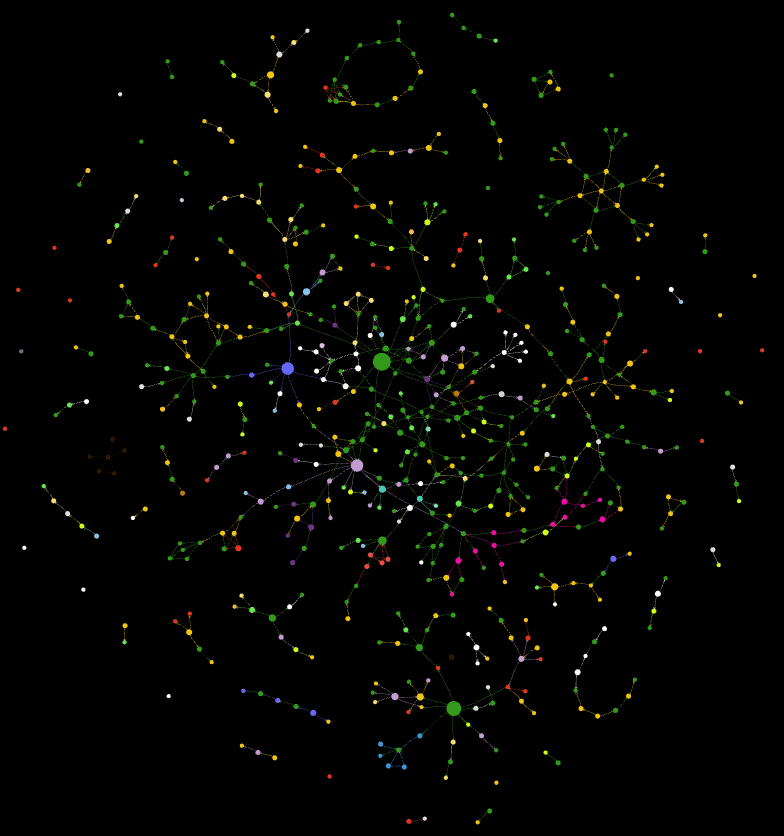
\includegraphics[width=130mm, keepaspectratio]{img/afantzazie_production_dataset_641_nodes.png}
    \caption{The entire dataset of afantazie.cz (641 nodes) in a single time window}
    \label{obr:afantzazie_production_dataset_640_nodes}
\end{figure}

\subsubsection{Animated edges}
This feature is currently unused and unparametrized (instead it is just commented out in the source code) but is worth mentioning.
Instead of the curved arrows used by default these edges consist of a series of sections flowing from referenced thought to its replies. This helps to visualize the flow of time from older to newer posts.

You can see screenshot of this feature in figure \ref{obr:afantazie_animated_edges}.
It remains unused as the animation has small visual artifacts but once fixed could be added as an optional setting.

\section{Graph View Performance}

The graph can handle the entire CitHep dataset and thanks to dynamic loading could handle even larger graphs.
On figure \ref{obr:afantazie_cithep_highlighted_thought} you can see a highlighted thought from the \gls{cithep_dataset} dataset.

To achieve this we wrote a C\# script to import the CitHep data files into Aphantasia database.
In graph view we used the same parameter settings we used for the much smaller graphs in \gls{production} environment
which at the time consisted of around 600 and 150 thoughts respectively.
To our surprise the resulting graph behaved well and except for increased tendency to jitter the CitHep graph view was smooth and stable.
The only parameter we had to change was neighborhood \gls{BFS} depth - from three down to just one.
CitHep graph is bigger and much more interconnected than the small production graphs so even at depth two
the graph walk feature often resulted in unreasonable amount of on-screen nodes.

\subsection{Limits of the Graph View}

In the previous chapter, in figure \ref{obr:afantazie_cithep_3k}, we have seen how Aphantasia handles 3000 nodes. 

The application is not meant to display large graphs at once, but out of curiosity we tried to render as many thoughts as possible.

First we tried to set the on-screen thought limit to 40000 (and thus load and render the entire CitHep dataset) and we were not able to fetch the data from the backend.
We are not sure why this happened but one possible explanation is that the API response is too large and either the server and/or the client were not able to handle it.

In the second test we set the on-screen thought limit to 10000 and we were able to fetch the data and render it.
The result was not unexpected - a big hairball of nodes and edges running at less than 1 frame per second.
See figure \ref{obr:afantazie_cithep_10000_on-screen-limit}.


\begin{figure}[p]
    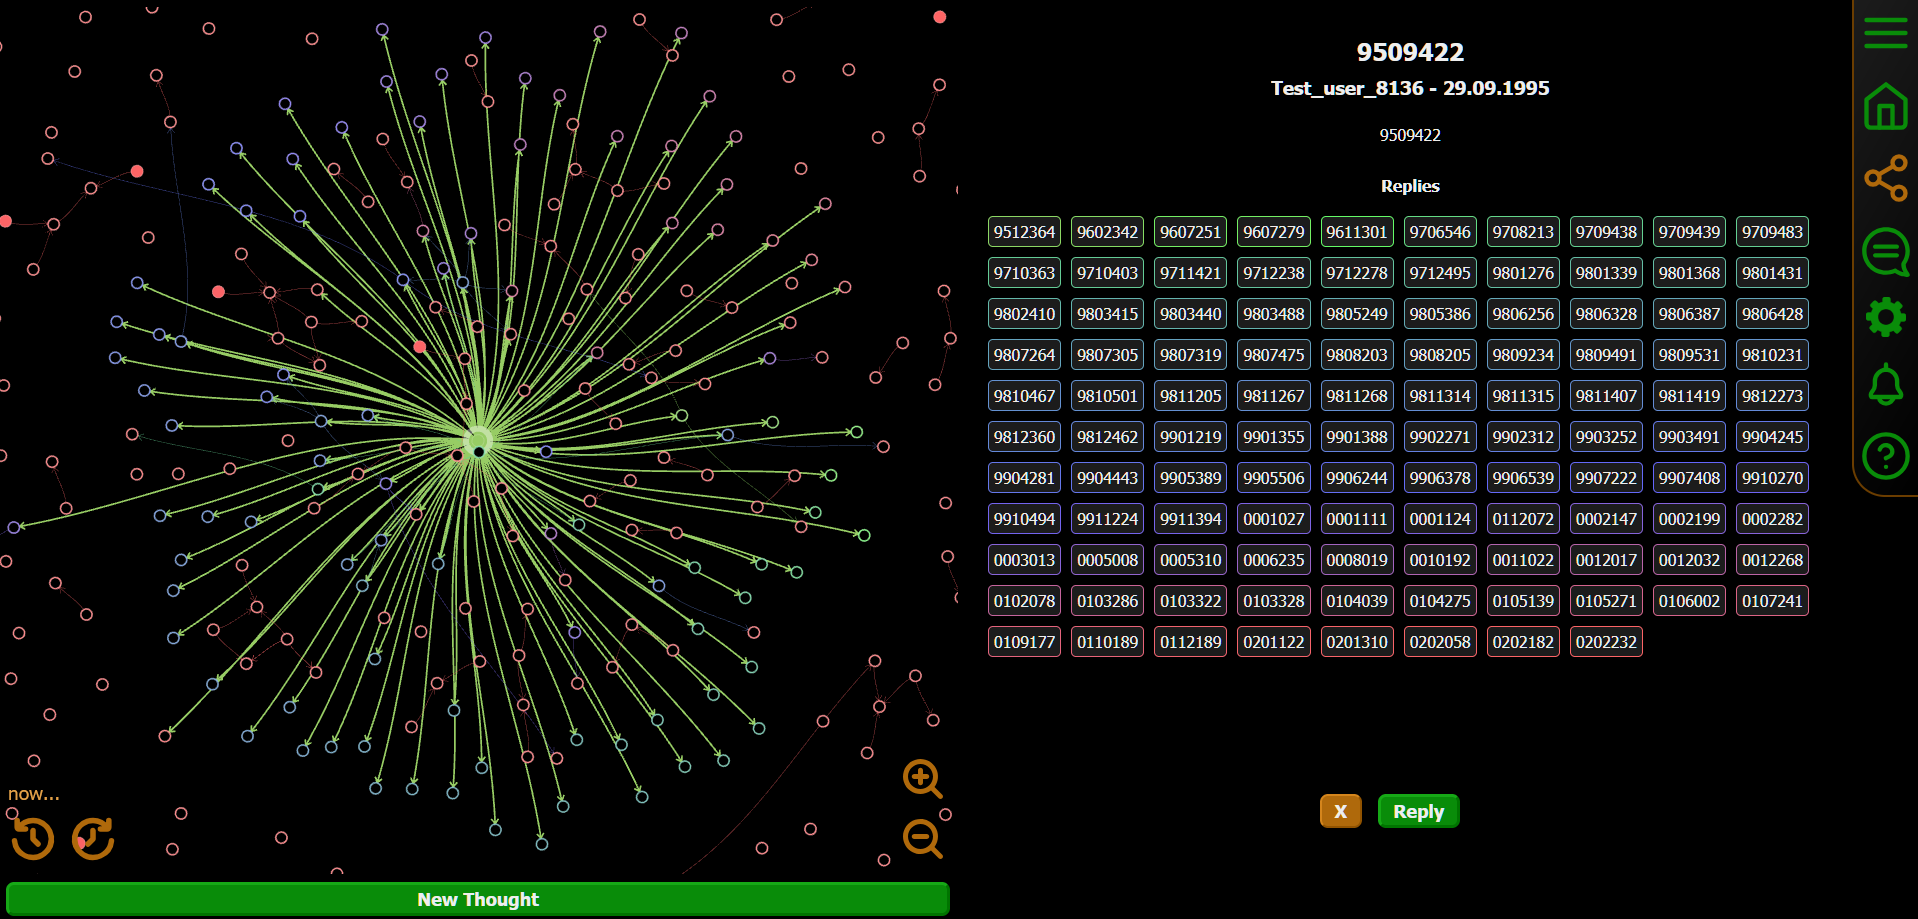
\includegraphics[width=130mm, keepaspectratio]{img/afantazie_cithep_highlighted_thought.png}
    \caption{A highlighted thought of the CitHep Dataset in Aphantasia}
    \label{obr:afantazie_cithep_highlighted_thought}
\end{figure}

\begin{figure}[p]
    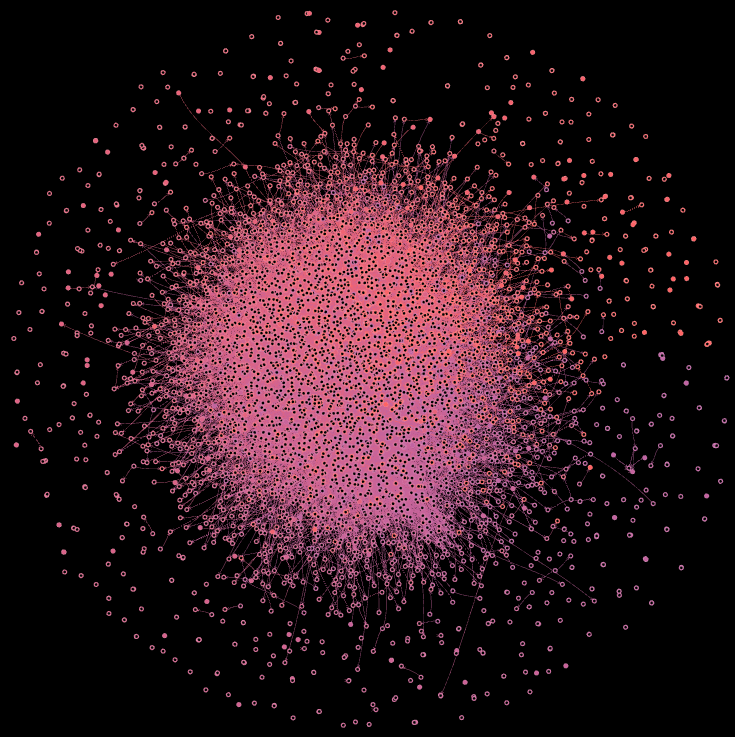
\includegraphics[width=130mm, keepaspectratio]{img/afantazie_cithep_10000_on-screen-limit.png}
    \caption{Cithep dataset rendered in Aphantasia with 10000 on-screen thought limit}
    \label{obr:afantazie_cithep_10000_on-screen-limit}
\end{figure}

From our tests we learned that Aphantasia's performance begins to degrade noticeably at around 400-700 on-screen thoughts limit and gradually drops to just few frames per second with the limit set to around 1,500.
These values are highly dependent on the connectivity of the data, with more connections leading to more computation time and thus lower performance.

\section{Deviation from the Original Plan}
Initially, we planned to implement a zoom-based dynamic loading and rendering system for large graphs.
However, we opted for a time-based and proximity-based approach (e.g., the time slider and neighborhood).

This decision was primarily driven by ease of implementation.
While zoom-based techniques remain valid, they are more complex and could have delayed progress.
The time slider naturally emerged as a consequence of the thoughts-on-screen limit, making zoom-based dynamic laoding a redundant feature to pursue further.

We also omitted filtering and searching functionalities.
These features are not critical, as graph exploration begins within a time window (latest or around a specific thought) and continues interactively.
The time saved was redirected to parameterizing and bug-fixing the graph view.
We still plan to implement these features in the future, as the architecture supports them and they will frther enhance the user experience.

\section{Future Development}

Although functional, Aphantasia remains an unpolished prototype.
Several significant issues and bugs require attention.
Some have already been mentioned in the previous sections, but the most pressing are:

\begin{itemize}
\item \textbf{Graph View Buttons}: Zoom and time slider controls often get stuck on mobile devices.
\item \textbf{Pinch Zoom}: This standard mobile feature is currently missing, making the graph view less intuitive on touch devices.
\item \textbf{Jitter}: While mostly resolved, occasional oscillations during node stabilization persist.
\item \textbf{Bugs}: Some notable issues include neighborhood thoughts persisting after graph view exit and re-entry. The Zustand graph store initialization needs an overhaul.
\item \textbf{Graph View Limits}: Neighborhood thoughts are not limited by the on-screen thoughts limit, thought positions cache has no size limit 
\item \textbf{Tutorial}: A tutorial is necessary to help new users understand the application, especially those unfamiliar with graph visualization.
\item \textbf{Backend Validation}: The backend’s Create Thought endpoint has a redundant links parameter, leading to potential inconsistencies when used programmatically.
\item \textbf{Notifications}: The current system lacks paging and cannot distinguish between read and unread notifications.
A dedicated notifications table could address these issues and enable more diverse notification types.
\end{itemize}

Despite these issues, Aphantasia has met and exceeded many of our expectations and the prototype stands on solid grounds, ready for further development.
After refining the prototype and fixing the problems, we plan to add new features and improvements, such as:
\begin{itemize}
\item Streamlining UI and UX
\item Filtering/Search
\item More graph algorithms besides \gls{FDL}
\item Email Verification
\item Password Reset functionality
\end{itemize}

\section{User Feedback}
We advertised the application on Reddit, sharing both the Czech and English versions across several subreddits.

Most comments were positive, praising the application’s concept and the experience of exploring thoughts
with one user describing the experience as feeling like an “archeologist” uncovering ideas. \xxx{cit?}

Negative feedback focused on the lack of practicality, outdated UI, and occasional bugs.
Users also suggested missing features such as pinch zoom, image posting, a better landing page, and filtering.
Browser compatibility issues were mentioned as well.

The feedback was mostly constructive and we are grateful for it.
It helped us hone on the experience users already found fun and stimulating, specifically interaction and exploration.
However, some users admitted they did not understand the application, highlighting the need for a proper tutorial.

\section{Aphantasia Versus Related Software}

Ideologically Aphantasia is closest to Obsidian.
There is of course an obvious difference between the two - Obsidian is local note-taking system with graph view while Aphantasia is an online social experience based on graph view.
Both are however meant for general audience and their graph views bare a similarity.

Compared to Gephi and Cytoscape.js Aphantasia has lower performance on large graphs rendered at once.
However thanks to Time slider and Graph walk features it can handle much larger datasets in an intuitive way.
The dynamic loading could in theory handle millions of nodes. In such case the main limiting factor would be the performance of the backend and the database.

Finally in table \ref{tab:comparison_2} we added Aphantasia to the comparison table from the first chapter.

\begin{table}[ht]
    \centering
    \caption{Comparison of Obsidian, Gephi, Cytoscape.js and Aphantasia}
    \label{tab:comparison_2}
    \begin{tabularx}{\textwidth}{|l|X|X|X|X|}
      \hline
      \textbf{}                     & \textbf{Obsidian}       & \textbf{Gephi}                      & \textbf{Cytoscape}                & \textbf{Aphantasia} \\ \hline
      \textbf{Use-case}             & note-taking             & data analysis and visualization     & graph visualization in browser    & social network \\ \hline
      \textbf{Target}               & general                 & researchers,                        & web                               & general \\ 
      \textbf{Userbase}             &  audience               & technical users                     & developers                        & audience, graph enthusiasts \\ \hline
      \textbf{User}                 & easy to use             & technical,                          & program-                          & intuitive, \\
      \textbf{Experience}           &                         & steep learning curve                & matic, mostly parametrization     & slight learning curve\\ \hline
      \textbf{3 000 nodes}          & slow                    & stable,                             & stable but                        & stable, \\ 
      \textbf{handling}             & indexing but smooth afterwards & smooth                              & visibly lower FPS                 & smooth, explorable \\ \hline
      \textbf{34 546 nodes}         & skipped as              & mostly                              & crashed                           & stable, \\ 
      \textbf{handling}             & indexing took too long  & stable, lower FPS while running FDL & immediately                       & explorable, slightly increased jitter \\ \hline
    \end{tabularx}
  \end{table}
\chapter{Documentation}
The remaining chapter is dedicated to the documentation of Aphantasia.

\section{User Documentation}
\label{chap:user_documentation}
All of the pages are accessible from the homepage and/or the collapsable navbar in the top right.

\subsection{Registering and Logging in}
While not logged in, only the graph view, about page, and welcome page are accessible.

To register, click on the register button on the home screen.
The registration requires selecting a unique username, email, and password.
The password has security requirements which are displayed immediately
after opening the form and in case of not meeting the criteria on submit.

To log in click on the login button on the homescreen. The login requires a username or email and password.

At this point, the email is not used anywhere and is only included in preparation for email verification functionality.

\subsection{Opening a Thought}
There are multiple ways to open a thought:
\begin{itemize}
  \item \textbf{New thoughts log on homepage} - On the homepage, there is a feed of the last three thoughts created on the website.
 Clicking on one of them will open the thought in graph view.
  
 Clicking on the "All Thoughts" button under the feed leads to the list of all thoughts.
  \item \textbf{Notifications} - The Notifications button and the bell icon in the navbar lead to the list of replies.
 Replies are thoughts of other users linked to any of the logged-in user's thoughts.
 Clicking on a reply opens the respective thought.
  \item \textbf{Graph view} - The main way to access thoughts is through the graph view. We will take a closer look at it in the next section.
  \item \textbf{Direct link} - Every thought has a unique ID which can be shared and accessed directly using the URL in format '/graph/\{thoughtId\}'.

 Example of the full URI leading to the thought with ID 1: https://aphantasia.io/graph/1
\end{itemize}

\subsection{Graph View}
To access the graph view, click the "Graph" button on the main page
or click on the graph icon in the navbar (three connected nodes).

In the graph view, the following controls are available:
\begin{itemize}
  \item \textbf{Mouse wheel or bottom right buttons} - Zooms in and out

 Once zoomed past a threshold, titles of the thoughts appear. (Figure \ref{obr:afantazie_floating_titles})
  \item \textbf{Draging the background} - Pans the viewport
  \item \textbf{Dragging a node} - Moves the grabbed thought around
  
 This is useful for customizing the layout, "untying" thoughts that are too close to each other or to speed up the process of the layout algorithm. 
  \item \textbf{Clicking a node} - Highlights a thought and switches to highlighted mode.
\end{itemize}

\subsubsection*{Highlighted Mode}

In default mode, the whole display is used to view the graph, and the user can interact with it as described above.
When a thought is accessed, the graph view switches to highlighted mode. (Figure \ref{obr:afantazie_mobile_graph_view})

In highlighted mode half of the screen gets dedicated to the highlighted thought preview and the other half to the graph view.

The graph view in highlighted mode shares almost all behavior with the default mode, with a few exceptions:
\begin{itemize}
  \item \textbf{Visual node highlight} - The currently opened thought is also visually highlighted by a white circle around it.
  \item \textbf{Visual edges highlight} - All edges connected to the opened thought are exaggerated in thickness and color while all other edges are dimmed.
  \item \textbf{Neighborhood thoughts} - On highlighting a thought, the application loads its neighborhood.
\end{itemize}
Every time a thought is selected, the viewport also smoothly centers on it.

The thought preview shows the title, author, time of creation, content with clickable links, and replies section.
Both the links in content and titles in the replies section are color-coded based on the author's selected color, and one-click will highlight the respective thought.
At the bottom of the preview there are Reply button and a close button (up icon on mobile and X on desktop).

\subsubsection*{Neighborhood Thoughts and Graph Exploration}

When a thought is highlighted, the application loads its neighborhood.
The neighborhood is defined as thoughts accessible through \gls{BFS} up to a given depth.
The currently used depth of the search is fixed at 3.

Some of the thoughts rendered on screen can be filled with black color. \ref{obr:afantazie_mobile_graph_view}
This indicates that some neighbors of the node are not visible on screen, and thus, the node is explorable.
  
\subsection{Creating a New Thought}

There are two ways to access the thought creation page:
\begin{itemize}
  \item \textbf{From the graph view} - Click on the "New thought" button at the bottom of the graph view.
  \item \textbf{From the thought preview} - Click on the "Reply" button at the bottom of the thought preview.
\end{itemize}

Both of these ways lead to the thought creation page (Figure \ref{obr:afantazie_thought_creation_page}).
The difference between them is that when accessed through the Reply button, the respective thought link
is automatically added to the content input.

The thought creation page consists of two text fields: Title and Content.

Both the title and content are required. Title has a minimum length of 1 character. The content's minimum length is 5 characters.
Both of these requirements are enforced by validation rules, and the user is notified by notification messages if the submit fails.

\subsubsection*{Referencing Other Thoughts}
When a link (or a reference) is added to a thought, it will be connected and attract the corresponding node in graph view.
Links can be added to the content field as a link with the format "[id](text)",
where id is the id of the thought and text is the text that will be displayed.
The text does not have to necessarily be the original title of the linked thought.

Adding links can be done in three ways:
\begin{itemize}
  \item \textbf{Manually} - By typing the link in the content field
  \item \textbf{By 'Add reference' button} - This button opens an overlay with a list of thought titles and a search bar.
 Click on a thought title to add it to the content at the cursor position.
  \item \textbf{Reply} - As mentioned, the Reply button in the graph view adds the link to the respective thought automatically.
\end{itemize}

Each thought can have up to five references.

\begin{figure}[h]\centering
  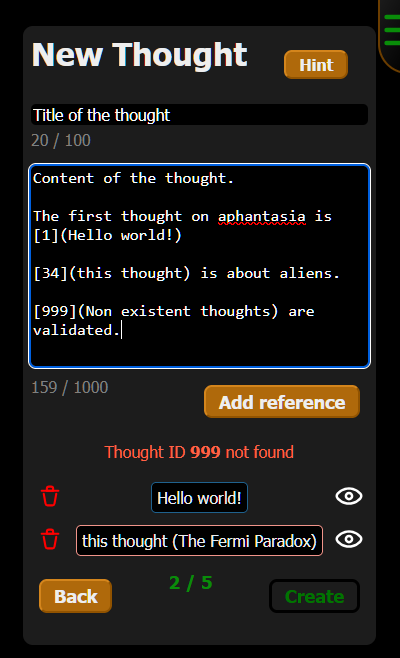
\includegraphics[width=100mm, keepaspectratio]{img/afantazie_thought_creation_page.png}
  \caption{Aphantasia - Thought creation page}
  \label{obr:afantazie_thought_creation_page}
\end{figure}

\subsection{Settings}
The settings page (Figure \ref{obr:afantazie_user_settings}) is accessible from the navbar by clicking on the gear icon or by clicking the "User settings" button on the homepage.
Currently, there are two settings that can be changed:
\begin{itemize}
  \item \textbf{On-screen thought limit} - This setting changes the maximum number of thoughts that are displayed on screen at once.
 The default value is 100. but can be changed to virtually any positive value.
  \item \textbf{Color} - This setting changes the color of users' thoughts in the graph view.
 There are predefined colors accessible by clicking the username but users are free to choose any color they like using a hexcode.
\end{itemize}

\begin{figure}[h]\centering
  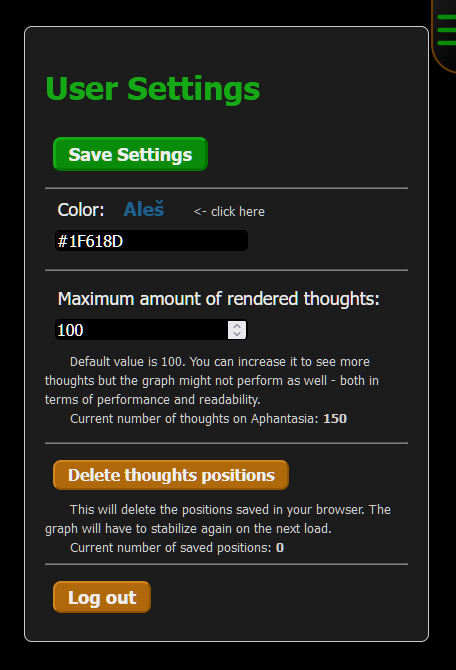
\includegraphics[width=100mm, keepaspectratio]{img/afantazie_user_settings.png}
  \caption{Aphantasia - User settings}
  \label{obr:afantazie_user_settings}
\end{figure}

Apart from these settings, there is also a \textbf{Log out} button
and \textbf{Delete thought positions} button, which erases positions of thoughts saved in the browser - forcing the graph to restabilize on the next load.

\section{Installation Guide}
Here we will look at how to set up and run both locally and how to deploy a public instance. 

\subsection{Running Aphantasia Locally}
To run Aphantasia locally, follow these steps:

\subsubsection{Database}
The database is necessary for the application to run.
It is set up using Entity Framework Core and PostgreSQL but one can choose any other database engine supported by EF Core.
To use a different database engine, install the necessary packages
and replace the \textbf{UseNpsql} methods in these two files appropriately:
\begin{itemize}
  \item \textbf{Afantazie.Data.Model/DatabaseContextProvider.cs}
  \item \textbf{Afantazie.Data.Model/DesignTimeDataContextFactory.cs}
\end{itemize}

With the database running the next step is to scaffold the database (ie. create the schema compatible with Aphantasia).
To do so, follow these steps:
\begin{enumerate}
  \item Add a file named \textbf{migrationsettings.json} in the root of project \textbf{Afantazie.Data.Model}.
  \item Add the following content to the file:
  \begin{lstlisting}
{
  "ConnectionStrings": {
    "DefaultConnection": "DATABASE CONNECTION STRING"
  }
}
  \end{lstlisting}
  \item Run the following command in the Data.Model project root:
  \begin{lstlisting}
    dotnet ef database update
  \end{lstlisting}
\end{enumerate}

The command should print the connection string provided in the migrationsettings.json and ask for confirmation.
If everything is correct, confirm the prompt by inputting "y", and the database should be created.

\subsubsection{Frontend}
Before running the frontend make sure to have Node.js with npm installed on the machine.
Open the root of the AfantazieWeb directory in a command line and run:
\begin{lstlisting}
 npm install
 npm run dev
\end{lstlisting}

The application will then be accessible at the address seen in the console output.
The language of the application can be changed by replacing \textbf{VITE\_LANGUAGE} to either 'en' or 'cz' inside the .env.development file.

\subsubsection{Backend}
Before running the backend, make sure to have .NET 8 SDK installed on the machine.

To run the Aphantasia backend, we recommend using Visual Studio and following these steps:
\begin{enumerate}
  \item Open the AfantazieServer.sln solution file in Visual Studio.
  \item Right-click the AfantazieServer project and click on Manage User Secrets.
  \item Copy the JSON with the connection string we provided in the database setup section and paste it into the secrets.json file.
  \item Set the AfantazieServer project as a startup project and run it.
\end{enumerate}

The project can be configured in the appsettings.Development.json file,
but it is not necessary for the application to run.

\subsubsection{Testing Data}
\label{sec:testing_data}
Apart from adding testing data manually throught the appliaction or directly inserting into the database one can also use the Afantazie.Tools project.
It is a .NET 8 console application inside the AfantazieServer solution
we created to help with various tasks regarding Afantazie development.
Among other things, it can generate random thoughts and users and add them to the database.

Before running the tool to generate thoughts, follow these steps:
\begin{enumerate}
  \item Host and scaffold a database as described above.
  \item Manually remove foreign key constraints from the ThoughtReferences table.
  \footnote{This is necessary as the tool doesn't generate the data optimally and violates these constraints.
 They can be added back after the import but it is not necessary for the application to run.}
  \item Create an appsettings.json in the root of the project.
 Its content should be the same as the migrationsettings.json shown above.
\end{enumerate}

Then, set the project as the startup project and run it.
Again the tool wil print the connection string and ask for confirmation after which it will present several options to pick from.
There are a few random data generators, but we recommend using option 3 - 'Generate random rainbow thoughts'.

This option will generate random clusters of thoughts where each generated thought has a set probability
of being linked to a thought in a different cluster.
User will then be asked for various parameters - fill them in and let the tool run.
Once it finishes, the database will be filled with random clustered thoughts
and users with unique colors across the color spectrum.

\subsection{Deploying Aphantasia}
To host Aphantasia publicly, we recommend using a Linux server (We used Debian 12.8).

Set up the database using the same steps as in the local setup.
The database can be hosted on the same server or on an external service (server or cloud).

\subsubsection{Frontend}
To prepare the frontend for deployment, first modify the .env.production file in the root of the AfantazieWeb directory.
Language and the backend URL need to be configured. Here is an example of our configuration:
\begin{lstlisting}
 VITE_LANGUAGE=cz
 VITE_URL=https://afantazie.cz
\end{lstlisting}

Then run the following commands in the root of the AfantazieWeb directory:
\begin{lstlisting}
 npm install
 npm run build
\end{lstlisting}

This will create a dist directory with the compiled frontend code.
Copy this code to a public directory on the server.

\subsubsection{Backend}
To deploy the backend, first, modify the app settings.Production.json file at the root of the AfantazieServer project.
Here is an example of our configuration:
\begin{lstlisting}
{
  "ApplicationLanguage": "cz",
  "JwtSecurityKey": "SECRET_KEY_HERE",

  "ConnectionStrings": {
    "DefaultConnection": "DATABASE CONNECTION STRING"
  }
}
\end{lstlisting}

In the JwtSecurityKey field, insert a secure string that will be used to sign JWT tokens.
In the ConnectionStrings field, insert the connection string to the database.
One can also change the language of the application by changing the ApplicationLanguage field.

We recommend using Visual Studio IDE to build the backend.
Create a new publish profile and set the target runtime to "Portable".
Then, publish the project in a directory and copy the files to the server.
Make sure to have the .NET 8 runtime installed on the server.

Finally, run the AfantazieServer.dll file with the following command:
\begin{lstlisting}
 dotnet AfantazieServer.dll
\end{lstlisting}

This way, the server will only run as long as the terminal is open.
To run the process in the background, we highly recommend using a program called \textbf{tmux} (another alternative is program \textbf{screen}).
Utilizing tmux makes it possible to run the server in the background.

\subsubsection{Nginx Configuration}
\label{sec:nginx_config}
As stated in Section \ref{sec:hosting} we use Nginx as a reverse proxy to reroute requests to the backend and to force the meta.json file to be always returned.
Here is how we set up the Nginx configuration file:
\begin{lstlisting}
server {
  server_name www.afantazie.cz afantazie.cz;
  root /www/hosting/afantazie.cz/www;

  index index.php index.html;

  include /etc/Nginx/sites-available/domains_conf/afantazie.cz.conf;
  if ($scheme != https)
  {
    return 308 https://$host$request_uri$is_args$args;
  }

  location /api {
    proxy_pass         http://127.0.0.1:5000;
    proxy_http_version 1.1;
    proxy_set_header   Upgrade $http_upgrade;
    proxy_set_header   Connection keep-alive;
    proxy_set_header   Host $host;
    proxy_cache_bypass $http_upgrade;
    proxy_set_header   X-Forwarded-For $proxy_add_x_forwarded_for;
    proxy_set_header   X-Forwarded-Proto $scheme;
  }

  location /hub {
    proxy_pass         http://127.0.0.1:5000;
    proxy_http_version 1.1;
    proxy_set_header   Upgrade $http_upgrade;
    proxy_set_header   Connection "Upgrade";
    proxy_set_header   Host $host;
    proxy_cache_bypass $http_upgrade;
    proxy_set_header   X-Forwarded-For $proxy_add_x_forwarded_for;
    proxy_set_header   X-Forwarded-Proto $scheme;
  }

  location /meta.json {
    add_header Cache-Control "no-cache, no-store, must-revalidate";
    expires -1;
  }
}
\end{lstlisting}

\section{Administrator Documentation}
This section is dedicated to the documentation of the Aphantasia administration.

\subsection{Backend}
To understand the architecture of the backend, see the detailed architecture description in Chapter \ref{sec:implementation_backend}.
There is not much to be done on the backend side apart from the initial setup and deployment.

The application has an active console logging, and one can see the activity on the site, including the number of currently active users,
thoughts currently being explored, as well as the creation of new thoughts.

\subsection{Frontend}
To understand the architecture of the frontend, see the detailed architecture description in Chapter \ref{sec:frontend_architecture}.


\subsubsection{Graph Layout Algorithm Parameters}
While running the Aphantasia's frontend publically it is important to keep in mind that the graph parametrization might become insufficient as the graph grows.
This is the main administration task on the frontend side - adjusting the graph layout algorithm parameters.

\label{sec:graph_layout_parameters}
\begin{itemize}
  \item \textbf{Forces}: Pull force, push force, and gravity force, including maximum allowed values and distance thresholds
  \item \textbf{Gravity On}: Boolean value that turns the gravity force on or off 
  \item \textbf{Link Distance}: Controls the spacing between connected thoughts
  \item \textbf{Momentum Dampening Divisor}: Forces acting on thoughts are divided by this number, resulting in a smoother with less jitter, but the graph will be slower to stabilize.
  \item \textbf{Stage Size}: The size of the simulation container
  \item \textbf{Radius Controls}: Base radius, size multiplier (how much larger more-referenced thoughts are), and maximum radius
  \item \textbf{Simulation Falloff Time}: Gradually slows down the \gls{GLA} after each user interaction (dragging or selecting thoughts and time sliding)
  \item \textbf{Frames with Overlap}: Allows newly appeared thoughts to overlap for a given amount of frames
  \item \textbf{Layout Caching Frequency}: Specifies how often the layout is saved to \gls{local_storage}
  \item \textbf{Node Mass}: Allows differently sized thoughts to have proportional influence on each other, with maximum and minimum values also parametrized
  \item \textbf{Backlinks Count Force Divisor}: Reduces forces acting on highly connected nodes
  \item \textbf{Edges Appearance}: Adjusts thickness and color of highlighted and unhighlighted edges (edges leading in or out of the currently highlighted node)
  \item \textbf{Animated Edges}: Turns on animated edges feature (seen in Figure \ref{obr:afantazie_animated_edges})
  \item \textbf{Frames With Less Influence}: New thoughts start with no influence over the simulation and gradually gain it over time
\end{itemize}

\chapter{Conclusion}

In this thesis, we have presented a novel approach to social network content presentation using a graph view
instead of the traditional infinite feed.
We discussed the motivation and the potential benefits it might bring.

We have implemented a proof-of-concept web application called Aphantasia, which utilizes such an approach, including 
a custom \gls{GLA} implementation and a rendering engine based on PixiJS.
During the development, we have solved several technical challenges regarding user management,
server-client communication, hosting, and, of course, graph rendering.

The finished application provides:
\begin{itemize}
    \item \textbf{Graph view} able to render several hundred nodes at once
    \item \textbf{Dynamic loading} ensuring the capability to explore large graphs in order of tens of thousands of nodes (and potentially much more)
    \item \textbf{User management} including registration and login
    \item \textbf{User interface}, including not just graph view but also pages with user settings, post creation form, chat
 and rudimentary notifications
   \item \textbf{Live preview} of the graph view
\end{itemize}

We are satisfied with the result and believe the application is a good starting point for further development.

We also believe that we have proven graph view as a viable alternative to interact with social media content,
provided that the content structure is allowed to have a form of \gls{DAG}.
Graph view might not be suitable for everyone, but it certainly attracts a niche of users who appreciate the exploration experience it provides.

%%% Bibliography
%%% Bibliography (literature used as a source)
%%%
%%% We employ biblatex to construct the bibliography. It processes
%%% citations in the text (e.g., the \cite{...} macro) and looks up
%%% relevant entries in the bibliography.bib file.
%%%
%%% See also biblatex settings in thesis.tex.

%%% Generate the bibliography. Beware that if you cited no works,
%%% the empty list will be omitted completely.

% We let bibliography items stick out of the right margin a little
\def\bibfont{\hfuzz=2pt}

\printbibliography[heading=bibintoc]

%%% If case you prefer to write the bibliography manually (without biblatex),
%%% you can use the following. Please follow the ISO 690 standard and
%%% citation conventions of your field of research.

% \begin{thebibliography}{99}
%
% \bibitem{lamport94}
%   {\sc Lamport,} Leslie.
%   \emph{\LaTeX: A Document Preparation System}.
%   2nd edition.
%   Massachusetts: Addison Wesley, 1994.
%   ISBN 0-201-52983-1.
%
% \end{thebibliography}


%%% Figures used in the thesis (consider if this is needed)
\listoffigures

%%% Tables used in the thesis (consider if this is needed)
%%% In mathematical theses, it could be better to move the list of tables to the beginning of the thesis.
\listoftables

%%% Abbreviations used in the thesis, if any, including their explanation
%%% In mathematical theses, it could be better to move the list of abbreviations to the beginning of the thesis.
\chapwithtoc{List of Abbreviations}

%%% Doctoral theses must contain a list of author's publications
\ifx\ThesisType\TypePhD
\chapwithtoc{List of Publications}
\fi

%%% Attachments to the thesis, if any. Each attachment must be referred to
%%% at least once from the text of the thesis. Attachments are numbered.
%%%
%%% The printed version should preferably contain attachments, which can be
%%% read (additional tables and charts, supplementary text, examples of
%%% program output, etc.). The electronic version is more suited for attachments
%%% which will likely be used in an electronic form rather than read (program
%%% source code, data files, interactive charts, etc.). Electronic attachments
%%% should be uploaded to SIS. Allowed file formats are specified in provision
%%% of the rector no. 72/2017. Exceptions can be approved by faculty's coordinator.
\appendix
\chapter{Attachments}

\section{First Attachment}

\end{document}
